%%% Local Variables:
%%% mode: latex
%%% TeX-master: t
%%% End:

%\documentclass[bachelor,nofonts]{thuthesis}
\documentclass[master]{thuthesis}
%\documentclass[doctor]{thuthesis}
% \documentclass[%
%   bachelor|master|doctor|postdoctor, % mandatory option
%   winfonts|nofonts|adobefonts, % mandatory only for bachelor and Linuxer
%   secret,
%   openany|openright,
%   arialtoc,arialtitle]{thuthesis}
% 当使用 XeLaTeX 编译时,本科生、Linux 用户需要加上 nofonts 选项;
% 当使用 PDFLaTeX 编译时,adobefonts 选项等效于 winfonts 选项(缺省选项)。

% 所有其它可能用到的包都统一放到这里了,可以根据自己的实际添加或者删除。
\usepackage{thutils}
\usepackage{lineno,hyperref}
% 你可以在这里修改配置文件中的定义,导言区可以使用中文。
% \def\myname{薛瑞尼}
\usepackage{amsmath}
\usepackage{comment}
\begin{document}

% 定义所有的eps文件在 figures 子目录下
\graphicspath{{figures/}}


%%% 封面部分
\frontmatter

%%% Local Variables:
%%% mode: latex
%%% TeX-master: t
%%% End:

% 中国海洋大学研究生学位论文封面
% 参考:中国海洋大学研究生学位论文书写格式20130307.doc

% 为避免出现错误,下面保留[清华大学学位论文模板原有定义无需修改],
% 请直接跳到后面[中国海洋大学学位论文模板部分请根据自己情况修改]。

%%%%%%%%%%%%%%%%%%%%%%[清华大学学位论文模板原有定义无需修改]%%%%%%%%%%%%%%%%%%%%%%%
\secretlevel{绝密} \secretyear{2100}

\ctitle{清华大学学位论文 \LaTeX\ 模板\\使用示例文档}
% 根据自己的情况选,不用这样复杂
\makeatletter
\ifthu@bachelor\relax\else
  \ifthu@doctor
    \cdegree{工学博士}
  \else
    \ifthu@master
      \cdegree{工学硕士}
    \fi
  \fi
\fi
\makeatother


\cdepartment[计算机]{计算机科学与技术系}
\cmajor{计算机科学与技术}
\cauthor{薛瑞尼} 
\csupervisor{郑纬民教授}
% 如果没有副指导老师或者联合指导老师,把下面两行相应的删除即可。
\cassosupervisor{陈文光教授}
\ccosupervisor{某某某教授}
% 日期自动生成,如果你要自己写就改这个cdate
%\cdate{\CJKdigits{\the\year}年\CJKnumber{\the\month}月}

% 博士后部分
% \cfirstdiscipline{计算机科学与技术}
% \cseconddiscipline{系统结构}
% \postdoctordate{2009年7月——2011年7月}

\etitle{An Introduction to \LaTeX{} Thesis Template of Tsinghua University} 
% 这块比较复杂,需要分情况讨论:
% 1. 学术型硕士
%    \edegree:必须为Master of Arts或Master of Science(注意大小写)
%              “哲学、文学、历史学、法学、教育学、艺术学门类,公共管理学科
%               填写Master of Arts,其它填写Master of Science”
%    \emajor:“获得一级学科授权的学科填写一级学科名称,其它填写二级学科名称”
% 2. 专业型硕士
%    \edegree:“填写专业学位英文名称全称”
%    \emajor:“工程硕士填写工程领域,其它专业学位不填写此项”
% 3. 学术型博士
%    \edegree:Doctor of Philosophy(注意大小写)
%    \emajor:“获得一级学科授权的学科填写一级学科名称,其它填写二级学科名称”
% 4. 专业型博士
%    \edegree:“填写专业学位英文名称全称”
%    \emajor:不填写此项
\edegree{Doctor of Engineering} 
\emajor{Computer Science and Technology} 
\eauthor{Xue Ruini} 
\esupervisor{Professor Zheng Weimin} 
\eassosupervisor{Chen Wenguang} 
% 这个日期也会自动生成,你要改么?
% \edate{December, 2005}

% 定义中英文摘要和关键字
\begin{cabstract}
  论文的摘要是对论文研究内容和成果的高度概括。摘要应对论文所研究的问题及其研究目
  的进行描述,对研究方法和过程进行简单介绍,对研究成果和所得结论进行概括。摘要应
  具有独立性和自明性,其内容应包含与论文全文同等量的主要信息。使读者即使不阅读全
  文,通过摘要就能了解论文的总体内容和主要成果。

  论文摘要的书写应力求精确、简明。切忌写成对论文书写内容进行提要的形式,尤其要避
  免“第 1 章……;第 2 章……;……”这种或类似的陈述方式。

  本文介绍清华大学论文模板 \thuthesis{} 的使用方法。本模板符合学校的本科、硕士、
  博士论文格式要求。

  本文的创新点主要有:
  \begin{itemize}
    \item 用例子来解释模板的使用方法;
    \item 用废话来填充无关紧要的部分;
    \item 一边学习摸索一边编写新代码。
  \end{itemize}

  关键词是为了文献标引工作、用以表示全文主要内容信息的单词或术语。关键词不超过 5
  个,每个关键词中间用分号分隔。(模板作者注:关键词分隔符不用考虑,模板会自动处
  理。英文关键词同理。)
\end{cabstract}

\ckeywords{\TeX, \LaTeX, CJK, 模板, 论文}

\begin{eabstract} 
   An abstract of a dissertation is a summary and extraction of research work
   and contributions. Included in an abstract should be description of research
   topic and research objective, brief introduction to methodology and research
   process, and summarization of conclusion and contributions of the
   research. An abstract should be characterized by independence and clarity and
   carry identical information with the dissertation. It should be such that the
   general idea and major contributions of the dissertation are conveyed without
   reading the dissertation. 

   An abstract should be concise and to the point. It is a misunderstanding to
   make an abstract an outline of the dissertation and words ``the first
   chapter'', ``the second chapter'' and the like should be avoided in the
   abstract.

   Key words are terms used in a dissertation for indexing, reflecting core
   information of the dissertation. An abstract may contain a maximum of 5 key
   words, with semi-colons used in between to separate one another.
\end{eabstract}

\ekeywords{\TeX, \LaTeX, CJK, template, thesis}
%%%%%%%%%%%%%%%%%%%%%%%%%%%%%%%%%%%%%%%%%%%%%%%%%%%%%%%%%%%%%%%%%%%%%%%%%%%%%%%%

%%%%%%%%%%%%%%%%%%[中国海洋大学学位论文模板部分请根据自己情况修改]%%%%%%%%%%%%%%%%%%%
% 中国海洋大学研究生学位论文封面
% 必须填写的内容包括(其他最好不要修改):
%   分类号、密级、UDC
%   论文中文题目、作者中文姓名
%   论文答辩时间
%   封面感谢语
%   论文英文题目
%   中文摘要、中文关键词
%   英文摘要、英文关键词
%
%%%%%[自定义]%%%%%
\newcommand{\fenleihao}{}%分类号
\newcommand{\miji}{}%密级 
                    % 绝密$\bigstar$20年 
                    % 机密$\bigstar$10年
                    % 秘密$\bigstar$5年
\newcommand{\UDC}{}%UDC
\newcommand{\oucctitle}{基于多特征多分类器组合的海洋浮游动物图像\protect\\分类研究}%论文中文题目
\ctitle{基于多特征多分类器组合的海洋浮游动物图像分类研究}%必须修改因为页眉中用到
\cauthor{朱亚菲}%可以选择修改因为仅在 pdf 文档信息中用到
\cdegree{工学硕士}%可以选择修改因为仅在 pdf 文档信息中用到
\ckeywords{\TeX, \LaTeX, CJK, 模板, 论文}%可以选择修改因为仅在 pdf 文档信息中用到
\newcommand{\ouccauthor}{朱亚菲}%作者中文姓名
%\newcommand{\ouccauthor}{***}%外审时用到
%\newcommand{\ouccsupervisor}{姬光荣教授}%作者导师中文姓名
%\newcommand{\ouccdegree}{博\hspace{1em}士}%作者申请学位级别
%\newcommand{\ouccmajor}{海洋信息探测与处理}%作者专业名称
%\newcommand{\ouccdateday}{\CJKdigits{\the\year}年\CJKnumber{\the\month}月\CJKnumber{\the\day}日}
%\newcommand{\ouccdate}{\CJKdigits{\the\year}年\CJKnumber{\the\month}月}
\newcommand{\oucdatedefense}{           }%论文答辩时间
%\newcommand{\oucdatedegree}{2009年6月}%学位授予时间
\newcommand{\oucgratitude}{谨以此论文献给我的导师和亲人!}%封面感谢语
\newcommand{\oucetitle}{Marine zooplankton image classification based on combination of multiple features and multiple classifiers}%论文英文题目
%\newcommand{\ouceauthor}{Haiyong Zheng}%作者英文姓名
\newcommand{\oucthesis}{\textsc{OUCThesis}}
%%%%%默认自定义命令%%%%%
% 空下划线定义
\newcommand{\oucblankunderline}[1]{\rule[-2pt]{#1}{.7pt}}
\newcommand{\oucunderline}[2]{\underline{\hskip #1 #2 \hskip#1}}

% 论文封面第一页
%%不需要改动%%
\vspace*{5cm}
{\xiaoer\heiti\oucgratitude

\begin{flushright}
---\hspace*{-2mm}---\hspace*{-2mm}---\hspace*{-2mm}---\hspace*{-2mm}---\hspace*{-2mm}---\hspace*{-2mm}---\hspace*{-2mm}---\hspace*{-2mm}---\hspace*{-2mm}---~\ouccauthor
\end{flushright}
}

%\begin{comment}

\newpage 
%\mbox{} 
%\newpage

% 论文封面第二页
%%不需要改动%%
\vspace*{1cm}
\begin{center}
  {\xiaoer\heiti\oucctitle}
\end{center}
\vspace{10.7cm}
{\normalsize\songti
\begin{flushright}
{\renewcommand{\arraystretch}{1.3}
  \begin{tabular}{r@{}l}
    学位论文答辩日期:~ & \oucunderline{2.5cm}{\oucdatedefense} \\
    指导教师签字:~ & \oucblankunderline{5cm} \\
    答辩委员会成员签字:~ & \oucblankunderline{5cm} \\
    ~ & \oucblankunderline{5cm} \\
    ~ & \oucblankunderline{5cm} \\
    ~ & \oucblankunderline{5cm} \\
    ~ & \oucblankunderline{5cm} \\
    ~ & \oucblankunderline{5cm} \\
    ~ & \oucblankunderline{5cm} \\
  \end{tabular}
}
\end{flushright}
}

\newpage 
%\mbox{} 
%\newpage

% 论文封面第三页
%%不需要改动%%
\vspace*{1cm}
\begin{center}
  {\xiaosan\heiti 独\hspace{1em}创\hspace{1em}声\hspace{1em}明}
\end{center}
\par{\normalsize\songti\parindent2em
本人声明所呈交的学位论文是本人在导师指导下进行的研究工作及取得的研究成果。据我所知,除了文中特别加以标注和致谢的地方外,论文中不包含其他人已经发表或撰写过的研究成果,也不包含未获得~\oucblankunderline{7cm}(注:如没有其他需要特别声明的,本栏可空)或其他教育机构的学位或证书使用过的材料。与我一同工作的同志对本研究所做的任何贡献均已在论文中作了明确的说明并表示谢意。
}
\vskip1.5cm
\begin{flushright}{\normalsize\songti
  学位论文作者签名:\hskip2cm 签字日期:\hskip1cm 年 \hskip0.7cm 月\hskip0.7cm 日}
\end{flushright}
\vskip.5cm
{\setlength{\unitlength}{0.1\textwidth}
  \begin{picture}(10, 0.1)
    \multiput(0,0)(0.2, 0){50}{\rule{0.15\unitlength}{.5pt}}
  \end{picture}}
\vskip1cm
\begin{center}
  {\xiaosan\heiti 学位论文版权使用授权书}
\end{center}
\par{\normalsize\songti\parindent2em
本学位论文作者完全了解学校有关保留、使用学位论文的规定,并同意以下事项:
\begin{enumerate}
\item 学校有权保留并向国家有关部门或机构送交论文的复印件和磁盘,允许论文被查阅和借阅。
\item 学校可以将学位论文的全部或部分内容编入有关数据库进行检索,可以采用影印、缩印或扫描等复制手段保存、汇编学位论文。同时授权清华大学“中国学术期刊(光盘版)电子杂志社”用于出版和编入CNKI《中国知识资源总库》,授权中国科学技术信息研究所将本学位论文收录到《中国学位论文全文数据库》。
\end{enumerate}
(保密的学位论文在解密后适用本授权书)
}
\vskip1.5cm
{\parindent0pt\normalsize\songti
学位论文作者签名:\hskip4.2cm\relax%
导师签字:\relax\hspace*{1.2cm}\\
签字日期:\hskip1cm 年\hskip0.7cm 月\hskip0.7cm 日\relax\hfill%
签字日期:\hskip1cm 年\hskip0.7cm 月\hskip0.7cm 日\relax\hspace*{1.2cm}}

%\end{comment}

\newpage 
%\mbox{} 
%\newpage

\pagestyle{plain}
\clearpage\pagenumbering{roman}

% 中文摘要
%%[需要填写:中文摘要、中文关键词]%%
\begin{center}
  {\sanhao[1.5]\heiti\oucctitle\\\vskip7pt 摘\hspace{1em}要}
\end{center}
{\normalsize\songti

  \indent
海洋覆盖了地球上约70\%左右的面积,对人类有着重要而深远的影响,能够为人类创造巨大的经济、社会、环境效益。海洋生态系统是一个结构复杂的大系统,浮游动物是其中的重要一员,其生物量、种群结构以及群落多样性对海洋生态系统、海洋生物地球化学循环、海洋环境以及全球气候变化研究都起着重要的作用。

随着浮游生物光学成像系统的不断发展,海量的浮游动物图像资料涌现出来,为浮游动物的监测和分类带来了挑战。本论文主要针对浮游动物图像分类技术中的特征提取和分类器设计两个关键步骤进行了分析和研究,提出了一种基于多特征多分类器组合的浮游动物图像分类方法,主要研究工作如下:

\begin{enumerate}
\item 以混淆矩阵中的分类准确率指标作为评价函数,对由图像处理领域常用特征、各种分类竞赛中采用的经典特征、浮游动物形态特征等组成的特征集进行特征选择,最终挑选出适用于浮游动物图像的三类特征,分别为PkID软件中的22个特征、局部二值模式特征、内距离形状上下文特征。
\item 对于挑选出的三类特征,分别对其采用不同的分类算法进行分类,将分类结果用交叉验证方法进行评价,根据评价结果挑选出适用于每类特征的分类算法,得到三个分类器。
\item 单个分类器对浮游动物图像分类可能存在一定的片面性,分类性能不能达到最佳,对此,我们提出了一种基于多特征多分类器组合的浮游动物图像分类方法,从而能够综合不同分类器的信息,提高分类准确率。
\end{enumerate}

我们在包含13类浮游动物的数据集上进行了对比实验,证明了本文的算法与其它浮游动物分类方法相比在分类准确率上有明显的提高,对于浮游动物分类是有效和可行的。
}
\vskip12bp
{\xiaosi\heiti\noindent
关键词:\hskip1em 海洋浮游动物; 图像分类; 机器学习; 多特征多分类器组合}

\newpage 
%\mbox{} 
%\newpage

% 英文摘要
%%[需要填写:英文摘要、英文关键词]%%
\begin{center}
  {\sanhao[1.5]\heiti\oucetitle\\\vskip7pt Abstract}
\end{center}
{\normalsize\songti

The ocean occupies about 70\% of the earth surface, producing significant economic, social and environmental benefits for human beings. Marine ecosystem is a complicated system,  in which zooplankton is an important member. Marine zooplankton biomass, population structure and community diversity play an important role in marine ecosystems, marine biogeochemical cycles, marine environment and global climate change research.

With the development of marine plankton optical imaging system, a tremendous amount of zooplankton images sprang up, which challenges the monitoring and classification of zooplankton. The thesis mainly focuses on the feature extraction and classifier design steps in zooplankton image classification, presenting a new zooplankton image classification method based on combination of multiple features and multiple classifiers.  Main tasks are as follows:

\begin{enumerate}
\item The classification accuracy indicator of confusion matrix is taken as the evaluation function for feature selection from the feature sets, which is composed of the most frequently used features in image processing fields, classic features in various classification competitions and zooplankton configuration features. We finally select three suitable types of features for zooplankton images: 22 features in PkID, local binary pattern and inner-distance shape context.
\item For each of the three types of features we choose, we apply different classification algorithm for it, and then use cross validation for evaluation. According to the evaluation results, we can select the most proper classification algorithm for each feature type and achieve three classifiers.
\item Single classifier for zooplankton classification has some certain one-sidedness, and the classification performance may not get the best. We propose a method based on combination of multiple features and multiple classifiers, thus can combine the information of different classifiers and improve the performance.
\end{enumerate}

The performance comparison on zooplankton dataset with 13 categories validates that the proposed method has an obvious increasement on classification accuracy compared with other methods in zooplankton image identification. It is feasible and effective in zooplankton classification.
}
\vskip12bp
{\xiaosi\heiti\noindent 
\textbf{Keywords:\enskip marine zooplankton, image classification, machine learning, combination of multiple features and multiple classifiers}}
%%%%%%%%%%%%%%%%%%%%%%%%%%%%%%%%%%%%%%%%%%%%%%%%%%%%%%%%%%%%%%%%%%%%%%%%%%%%%%%%
%\newpage 
%\mbox{} 
%\newpage

% 设置 PDF 文档的作者、主题等属性
\makeatletter
\thu@setup@pdfinfo
\makeatother
%\makecover

% 目录
\tableofcontents

% 符号对照表
%\begin{denotation}

\item[HPC] 高性能计算 (High Performance Computing)
\item[cluster] 集群
\item[Itanium] 安腾
\item[SMP] 对称多处理
\item[API] 应用程序编程接口
\item[PI]	聚酰亚胺
\item[MPI]	聚酰亚胺模型化合物,N-苯基邻苯酰亚胺
\item[PBI]	聚苯并咪唑
\item[MPBI]	聚苯并咪唑模型化合物,N-苯基苯并咪唑
\item[PY]	聚吡咙
\item[PMDA-BDA]	均苯四酸二酐与联苯四胺合成的聚吡咙薄膜
\item[$\Delta G$]  	活化自由能~(Activation Free Energy)
\item [$\chi$] 传输系数~(Transmission Coefficient)
\item[$E$] 能量
\item[$m$] 质量
\item[$c$] 光速
\item[$P$] 概率
\item[$T$] 时间
\item[$v$] 速度
\item[劝  学] 君子曰:学不可以已。青,取之于蓝,而青于蓝;冰,水为之,而寒于水。
  木直中绳。(车柔)以为轮,其曲中规。虽有槁暴,不复挺者,(车柔)使之然也。故木
  受绳则直, 金就砺则利,君子博学而日参省乎己,则知明而行无过矣。吾尝终日而思
  矣,  不如须臾之所学也;吾尝(足齐)而望矣,不如登高之博见也。登高而招,臂非加
  长也,  而见者远;  顺风而呼,  声非加疾也,而闻者彰。假舆马者,非利足也,而致
  千里;假舟楫者,非能水也,而绝江河,  君子生非异也,善假于物也。积土成山,风雨
  兴焉;积水成渊,蛟龙生焉;积善成德,而神明自得,圣心备焉。故不积跬步,无以至千
  里;不积小流,无以成江海。骐骥一跃,不能十步;驽马十驾,功在不舍。锲而舍之,朽
  木不折;  锲而不舍,金石可镂。蚓无爪牙之利,筋骨之强,上食埃土,下饮黄泉,用心
  一也。蟹六跪而二螯,非蛇鳝之穴无可寄托者,用心躁也。\pozhehao{} 荀况
\end{denotation}



%%% 正文部分
\mainmatter
\chapter{绪论}

\section{课题的研究背景及意义}

地球上海洋的面积为3.6亿平方千米,约占地球表面总面积的71\%,海洋是地球上综合生产力最大的生态系统,对于经济的快速发展起到至关重要的作用。而在海洋当中,海洋浮游生物是数量最多、规模最庞大的生物种类,其主要包括浮游植物和浮游动物两大类。这些浮游生物,绝大多数个体较小(一般从几微米到几毫米),需要借助显微镜才能看清楚它们的身体构造,并且它们缺乏发达的运动器官,游动能力很弱。其中浮游植物属于初级生产者,是食物链的第一个环节,其数量变动对浮游植物群落结构和海洋生态环境的维持起着十分重要的作用。而浮游动物属于次级生产者,它的作用主要表现为:第一,它相当于在浮游植物和其它捕食者之间搭起一座桥梁,使能量可以顺利地由低向高传输,所以其在维持整个海洋中生物(包括浮游植物和鱼类等)数量方面起着举足轻重的作用。第二,浮游动物自身的尸体和摄食产生的粪便中含有有机碳元素,并且以这种形式将N、C、P等元素传输到深海,以丰富海洋的有机物元素。第三,栖息环境的变换会很大程度上地影响浮游动物,表现为群落的结构和和功能参数上的差异,而这些差异可以反应气候变化及海洋环境变化。第四,某些种类的浮游动物在较深水层大量密集,会形成深海散射层,阻碍或干扰水下声纳的信号传播,使声纳失效,因而,它们在国防军事中的作用也越来越受到人们的重视。

浮游生物监测的重点是调查其种类组成和数量分布,其中最重要的监测指标是“优势种类判定”及“密度计算”。传统的浮游生物监测主要是由工作人员在显微镜下观测样本,并对样本进行分类和计数。但是这种监测手段对浮游生物工作者的专业性要求较高,且需要大量人力、财力的支撑,识别速度较慢,无法达到实时分析的需求。在过去的几十年间,浮游生物成像系统得到了快速发展,从而可以在更精细的时间、空间尺度上对浮游生物进行研究。与此同时,为了有效解决由于浮游生物分类学人才稀缺而造成的种类鉴别滞后现象,越来越多的科研工作者投入到利用图像处理和模式识别技术进行浮游动物的自动分类与计数这一研究中,并且在目前阶段已经取得显著进展。

\section{浮游生物图像自动识别方法的国内外研究现状}

浮游生物图像自动识别技术的发展与成像系统的研究和改进密不可分,以下具体介绍这两类技术近年来在国内外的研究现状。

\subsection{浮游生物成像系统的发展}

传统的浮游生物图像通常是经过海洋调查采水取样,然后用显微镜对样本进行拍照而得。由于近几年摄像技术的不断提高和日益增长的海洋浮游生物实时监测的需求,使得新的浮游生物现场及光学成像系统不断涌现。

美国伍兹霍尔海洋研究所(WHOI)的科研团队研制的视频浮游生物录像机(Video Plankton Recorder,VPR)~\cite{davis2005three}可以近距离拍摄到浮游生物的影像,为研究浮游动物提供充足的样本;美国南佛罗里达大学研发的灰度图像颗粒探测系统(Shadowed Image Particle Platform and Evaluation Recorder,SIPPER)~\cite{remsen2004you}采用高速线扫描相机可对水下浮游生物连续成像;法国研制的水下颗粒物和浮游动物图像原位采集系统(Underwater Video Profiler,UVP)~\cite{davis1992video}采用传统的照明设备和经电脑处理的光学技术,可实现浮游动物和颗粒物的剖面观测以及浮游动物图像和颗粒物图像的原位采集;由美国流体成像技术公司研发生产的流式细胞摄像系统(FlowCam)~\cite{benfield2007rapid}能够从流体中快速检测出有机和无机悬浮体,具有连续成像拍照和流式计数功能。近年来,全息成像技术也逐步成为获取浮游生物图像的一种重要手段。英国数家科研机构联合开发一种新的全息成像样机(HOLOMAR)~\cite{Watson2004HoloMar},这款试验机是基于离轴技术,可以获得水下浮游生物图像,在水下$10^5cm^3$的容量内都能精确记录,并且最小分辨率能达到$10\mu m$。美国约翰霍普金斯大学于1999年研发了一款基于水下同轴激光的全息成像系统,在水下$732-1964cm^3$的体积内都能进行勘察,用电荷耦合器件替代了在暗室中进行全息干板记录~\cite{katz1999submersible}~\cite{pfitsch2005development}。

国内,厦门大学的戴君伟等人~\cite{戴君伟2006海洋赤潮生物图像实时采集系统}为采集海洋藻类生物图像研制了一种新的系统,该系统融合了流式细胞技术和常用的成像采集技术,能够快速获得图像数据。
国家海洋技术中心于连生等人~\cite{于翔2009水下全自动显微成像仪}于2009年研发的“水下全自动显微成像仪”,该仪器可以很好地对浮游生物进行拍照;浙江大学陈耀武、洪炎峰等~\cite{tan2012实时浮游生物图像目标智能识别系统设计}开发的“实时浮游生物图像目标智能识别系统”能够对海洋水体中的目标生物进行实时连续走航大面积探测和图像采集;中国海洋大学于新生、周章国等~\cite{zhou2008design}开展了基于光学成像的浮游生物实时在线监测系统研究。综上,在对海洋浮游生物成像的研究中,不断涌现的采集系统保证了充足的研究资源,使基于图像处理的浮游生物研究更具有发展前景。

\subsection{浮游生物图像自动识别技术的发展}

海洋浮游生物的种类多种多样,对这么多的物种进行分类是一项非常繁重的任务。传统的浮游生物识别方法一般是人工地依据形态、尺寸、纹理、颜色等特征进行分类,再根据医学和化学上的一些知识进行进一步判定。但是这种人工识别方法存在一些明显的缺点:首先是对专业性要求较高,工作量大,效率低,浮游生物工作者在识别过程中易疲劳,从而难以保证海洋浮游生物监测的实时性和准确性。近年来发展了很多用来鉴定浮游生物的新技术,例如光谱法、流式细胞术等,但这些方法大多过程繁琐,严重依赖于浮游生物的生理状态,同时仪器昂贵,费用消耗较多。而目前利用数字图像处理技术进行浮游生物自动分类的方法,与其他方法相比,研究成本较低,可以实现精确的种属识别,因而越来越受到重视。

在对海洋浮游生物进行监测的技术中,数字图像处理这一方法的使用可以追溯到1970年,当时计算机处理能力有限,加上光学成像传感器的灵敏度和分辨率较低,对图像只能进行一些基本的信息获取。例如,利用模式识别方法对显微镜下的浮游动物进行简单的计数、尺寸度量和分类~\cite{jeffries1984automated}。近几年,图像处理技术快速发展,计算机性能不断提升,利用图像处理技术进行浮游生物的分类识别也取得了长足的进展。

二十世纪末期,欧洲自动硅藻识别和分类项目建立了自己的硅藻图像数据库并实现了硅藻的自动判识,其使用的方法包括数字图像处理和模式识别。基于 ADIAC 项目,硅藻显微图像分析取得一系列进展~\cite{hicks2006model}~\cite{dimitrovski2012hierarchical}~\cite{wilkinsondiatom}。此外,Embleton 等~\cite{embleton2003automated}结合计算机图像分析利用多层感知器(MLP)神经 网络方法实现 4 种浮游植物自动计数。Culverhouse 等~\cite{culverhouse2003experts}基于人工神经网络进行 6 种甲藻分类。Blaschko 等~\cite{blaschko2005automatic}采用图像分割、特征提取和模式识 别方法实现 12 类浮游生物自动识别。Davis 和 Hu~\cite{hu2006accurate}利用形状和纹理特征采用神经 网络和支撑向量机进行 6 类浮游生物自动识别及丰度估计。Sosik 和 Olson~\cite{sosik2007automated}通过边缘检测等图像处理后提取尺寸、形状、纹理等特征再采用支撑向量机完成 22 类浮游 植物自动分类和丰度估计。Hense 等~\cite{hense2008use}结合荧光图像进行浮游生物结构分析 (PLASA)。Verikas 等~\cite{verikas2012phase}结合相位一致性圆形目标检测、随机优化目标轮廓确定 以及支撑向量机和随机森林分类方法实现微小原甲藻细胞目标的检测和识别。腰鞭毛虫分类项目中,研究者们利用形状和纹理特征,采用人工神经网络分类算法对不同种类的腰鞭毛虫进行了分类~\cite{culverhouse2003expert}。法国国家科学院的研究者们对浮游动物进行了位置特征、尺寸特征、灰度特征、形状特征、生物统计特征以及其它自定义特征的提取,并提供了7种常见的分类算法供选用,实现了对浮游动物的分类识别,识别准确率达到80\%左右。Ellen等人~\cite{Quantifying2015Ellen}对已有的机器学习方法进行了研究,能够对浮游动物分类问题的算法选择、性能调整等提供指导,从而最大限度地提高分类准确率。

与国外相比,国内在利用数字图像处理技术来实现浮游生物的分类识别上起步较晚,因而不管在在研究时间还是研究深度上都是有很大的距离的,并且大多数项目的研究对象都是针对浮游植物(如藻类)的。王明时等人~\cite{王明时2004显微图像分析技术在赤潮生物识别中的应用}首先使用阈值法和形态学法对已有的赤潮生物显微图像进行处理,在图像中得到单个的浮游生物个体,再对这些个体的灰度和轮廓特征进行提取,最终完成分类识别。汪振兴等人~\cite{汪振兴2007赤潮藻类图像自动识别的研究}在对藻类图像的分类识别当中,提取了纹理和形状两种类型的特征,并采用了人工神经网络分类算法训练出分类器,实现了对赤潮藻的自动识别。骆巧琦等人首先对硅藻样本进行了采集,然后通过双轮廓叠加法对采集到的图像进行了分割,再提取了几何描述特征和形状描述特征,经过人工神经网络算法进行训练,最终得到精确的分类器~\cite{骆巧琦2011基于形状特征的硅藻显微图像自动识别}。魏雅娟等提取了基本的形态特征和纹理特征,采用支持向量机作为分类算法,实现了浮游动物图像的自动识别~\cite{魏雅娟2013暗视场浮游动物图像自动识别方法研究}。

综上所述,目前国内外基于图像技术的浮游生物分析主要在于浮游生物的目标识别和计数,且主要呈现出以下特点:

\begin{enumerate}
\item 就研究对象而言,国内外关于浮游动物分类识别的研究明显少于对浮游植物(如藻类)的识别研究。

\item 就研究范围而言,大多集中在某一个种类或者少量几个类别。

\item 就目标表示的特征提取而言,大多数研究方法选择外部形状特征和纹理特征作为浮游生物特征提取和描述,而多数浮游生物纹理特征并不明显,难以作为分类特征,且对特征没有进行有效研究与分析。

\item 就分类技术而言,逐渐趋于使用机器学习算法作为分类器,但一般使用单一的分类器得到分类结果,而没有考虑不同分类器分类结果的融合。
\end{enumerate}

\section{课题来源}

课题来源:国家自然科学基金青年科学基金项目“基于视觉注意结合生物形态特征的海洋浮游植物显微图像分析”(批准号:61301240)、国家自然科学基金项目“基于生物形态特征的中国海常见有害赤潮藻显微图像识别”(批准号:61271406)和中央高校基本科研业务费“海洋浮游动物原位探测与分析系统”(批准号:201562023)。

\section{论文组织结构安排}

本文总结了国际上现有的浮游动物图像分类方法,对其中基于机器学习的浮游动物图像分类算法进行了深入研究,并提出了基于多特征多分类器组合的浮游动物分类算法。本文的主要安排如下:

第一章为绪论部分,主要对浮游动物图像分类研究的背景、意义及国内外研究现状进行介绍,并对全文的主要安排进行了说明。

第二章介绍浮游动物图像分类的一些基础知识。详细介绍了用来进行分类的数据集以及利用机器学习方法进行浮游动物图像分类的过程,对浮游动物图像分类准确率最高的ZooScan系统进行了大致的描述,最后,说明了如何评价一个分类器性能的好坏。

第三章将图像处理和机器视觉领域一些常用的特征进行整理和总结,通过一定的评判标准进行特征选择,最终选取三类特征作为浮游动物图像的特征提取。

第四章简述了机器学习领域常用的分类技术,以分类准确率作为评判,设计适合各类特征的最优分类器。

第五章针对单一分类器存在分类片面性,提出了多特征多分类器组合的方法,详细介绍了算法的基本原理,并通过在包含13类浮游动物的数据集上进行实验证明了我们的方法的有效性。

第六章对全文的工作进行了总结,指出工作中存在的问题并对以后的工作提出了展望。
\chapter{浮游动物图像分类基础}

\section{机器学习分类技术}

利用机器学习方法对浮游动物图像进行分类的主要模块是图像预处理、特征提取、分类,主要步骤为:

(1)将浮游动物图像样本分为训练样本和测试样本两类,并建立实验所需的训练样本和测试样本数据;
(2)分别对训练样本和测试样本进行预处理;
(3)对训练样本进行特征提取,从中选择合适的特征信息构成特征向量;
(4)设计分类算法,通过支持向量机、随机森林、神经网络等方法设计分类器;
(5)将训练样本图像的特征输入到分类器,训练出分类模型;
(6)提取测试样本特征,并输入到分类模型中,输出测试样本的分类结果。具体见图~\ref{fig: ClassificationFlowchart}。

\begin{figure}[h] %插图
\centering
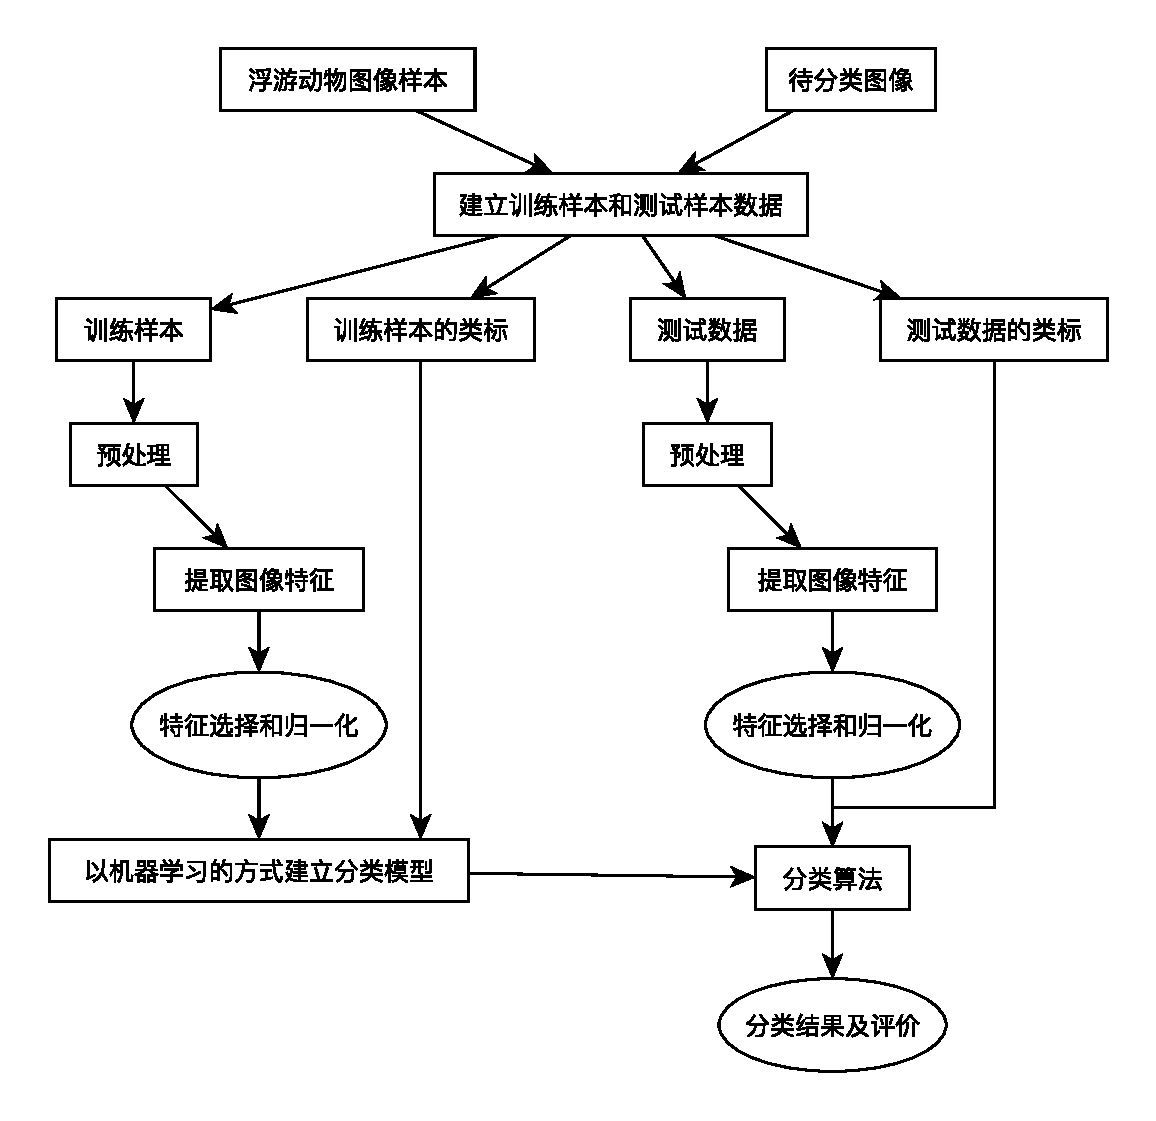
\includegraphics[width=0.6\textwidth]{ClassificationFlowchart.eps}
\caption{利用机器学习方法实现浮游动物图像分类的基本流程}
\label{fig: ClassificationFlowchart}
\end{figure}

\section{数据集}
\label{2.1}

自1949年起,加利福尼亚海洋渔业研究合作组织(California Cooperative Oceanic Fishery Investigation, CalCOFI)就开始对包括浮游生物在内的海洋生物进行采样~\cite{bograd2003calcofi},根据标准邦戈网络协议采集海洋中的浮游生物样本,然后立即保存起来。部分被保存的CalCOFI样本被连接到加利福尼亚对当前生态系统进行长期生态研究的网站上,并用ZooScan进行了扫描~\cite{gorsky2010digital}。得到的灰度图像质量较好,在对比度、噪声等方面都得到了精确控制。整个数据集包含的种类如表~\ref{表1}所示,其中每种类别图像所占比例见图~\ref{fig: ratio},以下对该数据集中的每一类别分别进行了详细说明和描述。

\begin{table}[htbp]
\centering
\caption{浮游动物数据集包含种类}
\begin{tabular}{|r|l|}
\hline
Appendicularia & 尾海鞘纲 \\
Bubble & 气泡 \\ 
Chaetognatha & 毛颚动物门 \\
Cladocera Penilia & 尖头溞属 \\
Copepoda & 桡脚类 \\
Decapoda & 十足目 \\
Doliolida & 海樽目 \\
Egg & 卵 \\
Fiber & 纤维 \\
Gelatinous & 明胶 \\
Multiple & 多个生物 \\
Pteropoda & 翼足目 \\
Nonbio & 非生物 \\
\hline
\end{tabular}
\label{表1}
\end{table}

\begin{figure}[!ht]
\centering
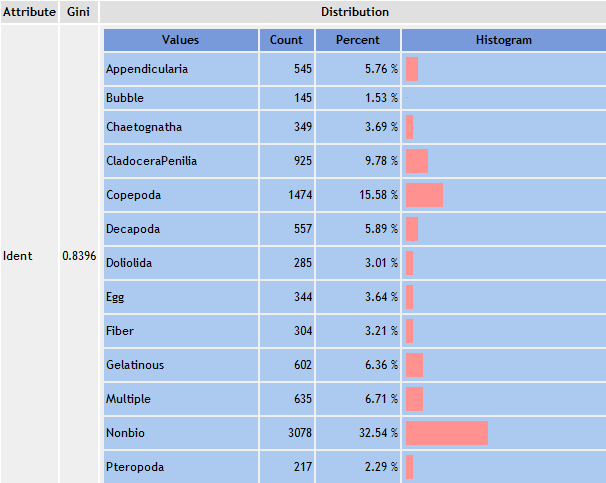
\includegraphics[width=0.6\textwidth]{每个类别所占比例.png}
\caption{数据集中每种类别的数目及所占比例}
\label{fig: ratio}
\end{figure} 

\begin{description}
    \item[Appendicularia(尾海鞘纲)] 属于脊索动物门,体型像蝌蚪,身体分为躯干和尾两部分。躯干较大且灰度较深,呈不太规则的椭圆形。尾部比躯干要长,长度大多小于5mm。尾部大致呈现两种形状:一种细长弯曲,另一种较粗(粗细甚至于头部差不多),呈现柳叶状。尾部的灰度相比于躯干较浅,轮廓不太清晰。

    \item[Bubble(气泡)] 非生物,圆形。气泡四周灰度深,中间灰度很浅,呈亮白色。

    \item[Chaetognatha(毛颚动物门)] 身体修长,可以明显看出身体分为头、躯干和尾3部分。头部略膨大,躯干与头连接处稍微缢缩为颈部,躯干较粗,轮廓清晰。尾部慢慢变窄,末端尖细。头部两侧各着生一列4~13根镰刀状、几丁质的颚毛。大小:最大成年成年个体长105mm,该类成年个体的长度一般都大于5mm。

    \item[Cladocera Penilia(Penilia,尖头溞属)] 属于节肢动物门,鳃足纲,枝角目,俗称水跳蚤。身体短小,有两条长长的触角。该类浮游动物身体中轴线的地方灰度较深(感觉类似人体的脊柱),这个颜色较深的中轴线上还有一条条纹理线连向边缘(就像人体脊柱上连着的骨骼)。由于运动,扫描得到的图像中浮游动物的中轴线并不是都在其身体中间。大小约为1mm左右。
    
    \item[Copepoda(桡脚类)] 属于节肢动物门,颚足纲,桡足类属于其下的一个亚纲。体形像泪珠,有大的触角。分为前体部和后体部,前体部较为宽大,后体部较为短小。前体部前体部由头和胸部组成,头部有两对触角,胸部有鄂足、五对胸足。后体部无附肢,由3—5节组成。最末的腹节称尾节,末端具1对尾叉,尾叉的末端有5根不等长的刚毛,常呈羽状。    
    
    \item[Decapoda(十足目)] 属于节肢动物门,软甲纲。又分为两类:Lucifer hanseni和Crab larvae。体躯延长呈虾形(腹部发达)或缩短扁圆呈蟹形(腹部化)。

    \item[Doliolida(海樽目)] 属于脊索动物门,樽海鞘纲。体型一般呈桶状,体壁最外是被囊层,其内层是外套膜。被囊层下有8~9条肌带环绕着体躯。由于该类浮游动物比较透明,因此在图像中灰度较浅,并且其桶状轮廓也不完整了,但最明显的是能看到大概7、8条环状的肌肉带,有的图像中还能看到内部器官。

    \item[Egg] 很多种类生物的卵。形状大致都呈圆形。有的卵整体灰度都很深;有的卵中间有一块灰度较深的区域,四周灰度较浅(结构像细胞)。由于是不同动物的卵,因此其灰度特征差异较大。

    \item[Fiber(纤维)] 非生物。弯曲的线状,有的纤维有分叉和交叉。该类图像中噪声较多,纤维的边缘也不是很规则。

    \item[Gelatinous(明胶)] 该类包括很多不同种类的胶状生物,它们体内都含有很高的水分。包括Aglaura(属于刺胞动物门)、Medusa(水母,属于刺胞动物门,水螅纲)、Siphonophora(管水母,属于刺胞动物门,水螅纲,管水母目)、Radiolaria(放射虫,属于原声动物门,辐足纲)和Salps(樽海鞘,属于脊索动物门Chordata,樽海鞘纲Thaliacea,纽鳃樽目Salpida)。其中水母大部分都有三个主要部位:圆伞状或是钟状(寺院里面敲得那种钟)的身体、触器和口腕。由于该类呈胶状,因此该类物体灰度整体较浅,边缘也不是十分清晰。大部分是水母,有小部分的樽海鞘(与海樽目形态很相似),小部分的放射虫。
        \item 其中水母也包括很多类,形态大致呈现以下几种:
            \begin{itemize}
            \item 一些水母身体呈现类似钟状(这里呈现钟状有长有短,有粗有细,还有的会发生一点弯曲),灰度较浅,内部有一块颜色较深的椭圆形区域。
            \item 一些水母也呈钟状,但内部没有颜色较深的椭圆形区域,整个身体灰度均匀。
            \item 还有的个头稍微偏小,形状有的类似圆形、像半个胶囊(应该是由于拍摄原因,有的拍到顶部,有的拍到侧面),体内有颜色较深的一个大点和几个小点。(可能是灯塔水母)
            \end{itemize}
        \item 放射虫:形状近似圆形(但由于整体灰度较浅,形状保存是完整),中间有一块灰度较深的区域,四周灰度较浅,可以看到淡淡的细纹从中心连接到边界。
        
    \item[Multiple(多个生物)] 由于浮游动物的重叠,导致分割过程中多个浮游动物被分割到一张图像上。
    
    \item[Pteropoda(翼足目)] 属于软体动物门,腹足纲。该类浮游动物灰度较深,形状总体都呈现一头宽一头窄。形状总体呈现三类:有的呈现象牙状,有点弯曲;有的较粗短,像一顶尖的小帽子;有的呈现细长的三角形状。
    
     \item[Nonbio] 非生物的集合。
\end{description}

\section{评价方法}

\subsection{混淆矩阵简介}
\label{CM}

在机器学习中,混淆矩阵(CM)是一种比较简单的对分类模型的性能进行评价的评估准则,主要用于比较分类结果和实际测得值。混淆矩阵是一个$n$行$n$列的矩阵,$n$代表类别的数量。矩阵的每一列代表预测的每一类的数量,每一行代表实际的每一类的数量。对角线上表示分类正确的每一类的数量。例如:有180个样本数据,这些数据实际分为3类,每类60个,分类结束后得到的混淆矩阵如表~\ref{ConfusionMatrixExample}所示。第一行说明类1的60个样本有53个样本分类正确,5个错分为类2,2个错分为类3。第一列说明类1有53个样本分类正确,类2的2个样本被错分为类1,类3没有样本被错分为类1。对角线上的数据表示,类1、2、3分别有53、55、59个样本被分类正确。
    
\begin{table}[ht]
\centering
\caption{混淆矩阵例子}
\begin{tabular}[c]{|c|c|c|c|}
\hline
 & 类1 & 类2 & 类3\\
 \hline
类1 & 53 & 5 & 2 \\
\hline
类2 & 2 & 55 & 3\\ 
\hline
类3 & 0 & 1 & 59\\ 
\hline
\end{tabular}
\label{ConfusionMatrixExample}
\end{table}

根据混淆矩阵可以导出以下几个参数:
\begin{itemize}
    \item true positives (TP):正样本被识别出的数量
    \item true negatives (TN):负样本被识别出的数量
    \item false positives (FP):负样本被错误分为正样本的数量
    \item false negatives (FN):正样本被错误分为负样本的数量 
    \item Accuracy:准确率,针对分类器的整个预测情况。
        \begin{displaymath}
            Accuracy=\frac{TP+TN}{TP+TN+FP+FN}
        \end{displaymath}
    \item {Error rate:误分类率,针对分类器的整体预测情况。}
        \begin{displaymath}
            Error rate=\frac{FP+FN}{TP+TN+FP+FN}
        \end{displaymath}
    \item {The true positive rate (TPR) :召回率,正样本被识别出的概率。}(文中和PkID中使用的评价参数)
        \begin{displaymath}
            TPR=\frac{TP}{TP+FN}
        \end{displaymath}
     \item The false positive rate (FPR):虚警率,负样本被错误分为正样本的概率。
        \begin{displaymath}
            FPR=\frac{FP}{FP+TN}
        \end{displaymath}
    \item The true negative rate (TNR):负样本被识别出的概率
        \begin{displaymath}
            TNR=\frac{TN}{FP+TN}
        \end{displaymath}

    \item The false negative rate (FNR) :漏警率,正样本被错误分为负样本的概率。
        \begin{displaymath}
            FNR=\frac{FN}{FN+TP}
        \end{displaymath}
    \item {False discovery rate (FDR):1-precision。}(文中和 PkID 中使用的评价参数)
        \begin{displaymath}
            FDR=\frac{FP}{FP+TP}
        \end{displaymath}
    \item Positive predictive value (PPV)
        \begin{displaymath}
            PPV=\frac{TP}{TP+FP}
        \end{displaymath}
    \item Negative predictive value (NPV)
        \begin{displaymath}
            NPV=\frac{TN}{TN+FN}
        \end{displaymath}
    
\end{itemize}

\subsection{混淆矩阵分类}

根据训练集和测试集的不同选取方式,混淆矩阵可以通过以下两种方式得到:
\begin{enumerate}
\item Re-substitution混淆矩阵       
当采用的测试集和训练集为同一个数据集时,得到的混淆矩阵叫做Re-substitution混淆矩阵。在这个过程中,用产生的分类器对测试集进分类时,得到的分类结果错误较少甚至可能没有错误,在进行评价时就会低估分类器的错误率。
\item 交叉验证混淆矩阵
采用交叉验证(交叉验证介绍见~\ref{Cross Validation})的方法得到的混淆矩阵就叫做交叉验证混淆矩阵。并且这里采用的训练集和测试集之间在样本上是没有重合的。首先将一个数据集分成$K$个相等的子集,用其中$K-1$个子集来训练产生分类器,用剩下的1个子集来进行测试,重复进行$K$次来构建混淆矩阵。
\end{enumerate}

\subsection{交叉验证}
\label{Cross Validation}
交叉验证是用来评价分类器的分类性能的一种方法,其基本步骤是是对原始图像集进行分组,然后选择没有交叉的两部分,一部分用作训练,一部分用作测试,用得到的混淆矩阵来评价分类器的性能好坏。

在机器学习的常见算法中,首要的步骤通常是将数据集分为训练集和测试集两个子集,其中训练集用来建立模型,而测试集则用来评价该模型对未知样本进行预测时的准确度,即泛化能力。如何将完整的数据集分为训练集跟测试集,必须遵守以下几条要点:
\begin{enumerate}
    \item 在训练分类器阶段用到的是训练集,不能使用测试集,训练完成后再在测试集上测试分类效果,将两者在分类器建立前后做到严格分离。
    \item 一般来说,训练集中图像数量要多于测试集,以保证训练出的分类器有效。
    \item 对于训练集和测试集,都必须做到对原始数据中每一类都均匀采样,不能过分偏向其中某几类,这样会导致训练出的分类器没有将所有类别的特点都考虑进去。
\end{enumerate}

常见的交叉验证形式有Holdout验证、$K$折交叉验证和留一验证三种,其中用的比较多是$K$折交叉验证。首先将原始的整个图像集平均分成$K$份,一般是随机挑选分配。每一次训练分别将其中一份作为训练集,另外的$K-1$份作为测试集,得到一个混淆矩阵,由于有$K$份,所以会进行$K$次训练和测试,得到$K$个混淆矩阵,将这$K$个混淆矩阵累加起来,就能得到$K$折交叉验证的混淆矩阵。$K$的取值通常大于等于2。在将图像集分成子集时由于是随机分配的,带有一定的随机性,所以在实际应用中,为了避免随机性对分类器效果的影响,我们通常会随机分配$n$次,将每一次得到的$K$折交叉验证的混淆矩阵进行叠加,得到最终的混淆矩阵。

本文中对分类结果采用$K$折交叉验证方式得到的混淆矩阵进行评价,其中$K$取值为2,$n$取值为5,对混淆矩阵计算Recall和1-Precision值,得到每一类的分类准确率和错误率,再对所有类别求平均,得到对整个数据集进行分类的分类准确率和错误率。

\section{ZooScan系统介绍}

利用机器学习方法进行浮游动物图像分类的方法有很多,目前取得最好的分类效果的是法国国家科学研究院研制的ZooScan系统~\cite{gorsky2010digital},受到该系统的启发,我们对其中的浮游动物图像特征提取和分类器设计两个关键环节进行了更深入的研究,从而对其进行了有效的改进,使分类准确率进一步提高。下面具体介绍ZooScan系统的主要组成部分。

\subsection{简介}

ZooScan Integrated System是由法国国家科学研究院Villefranche海洋实验室的Gorsky等人发明、Hydroptic公司生产的浮游动物样品图像扫描和处理系统,能够快速实现对液体中的浮游动物样品的扫描、计数、种类鉴定和生物量的测定,目前在国内和国外都影响很广。

ZooScan系统是由ZooScan、ZooProcess和Plankton Identifier (PkID)三个部分组成的,其中前者是系统的硬件部分,用来对液体中的浮游动物样品进行扫描,得到高分辨率的数字图像。后两者是软件部分,先对扫描得到的图像进行一些标准化处理,对个体的一些形态、几何、灰度等参数进行提取,然后利用一些基本的机器学习算法对特征进行训练,得到分类器,最终实现对浮游动物图像的分类识别。

\begin{figure}[!ht] %插图
\centering
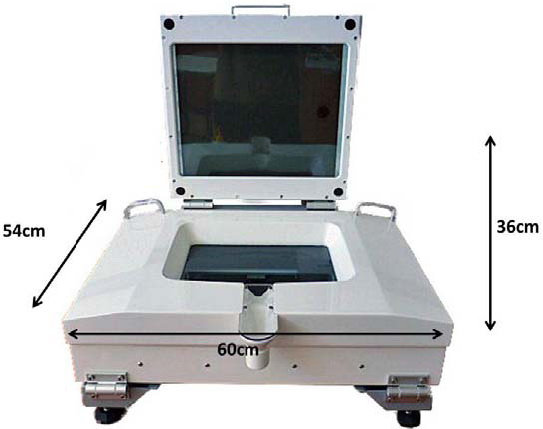
\includegraphics[width=0.4\textwidth]{ZooScan.jpg}
\caption{ZooScan主扫描区}
\label{fig: ZooScan}
\end{figure}

\subsection{硬件部分}

ZooScan系统的扫描设备分为了上下两个部分(图~\ref{fig: ZooScan}),为了能够扫描带液体的样本,对设备的防水性有较高的要求,ZooScan扫描系统在这方面作了很好地处理,其内部隔绝水的性能相当好。扫描设备的上面部分提供了两种功能,一是照明,二是进行光密度的检测。下面部分是扫描区域,即液体样本的放置地方。由于扫描时光是从空气进去水中,再从水中进入玻璃,要分两次完成在两种不同介质之间的穿透,因而在成像效果上会相应差一些,表现为图像分辨率的降低。针对浮游动物样本的不同尺寸,ZooScan系统提供了$1200dpi$和$2400dpi$两种分辨率以及$11cm\times24cm$和$15\times24cm$两种大小的扫描框以供选用。

\begin{figure}[!ht] %插图
\centering
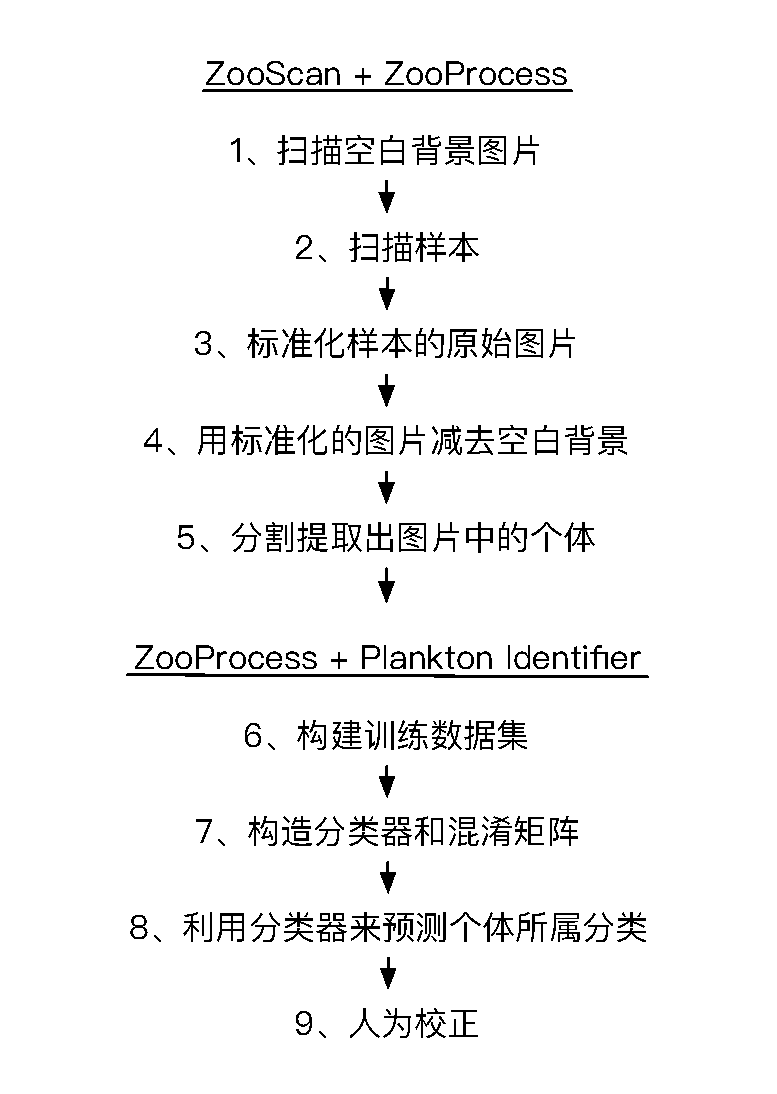
\includegraphics[width=0.4\textwidth]{ZooScanFlowchart.eps}
\caption{利用机器学习方法实现浮游动物图像分类的基本流程}
\label{fig: ZooScanFlowchart}
\end{figure}

\subsection{软件部分}
\label{2.3.3}

利用ZooScan系统对浮游动物进行扫描和分析的基本步骤如图~\ref{fig: ZooScanFlowchart}所示。最初的步骤是使用ZooProcess软件完成:(i)扫描空白背景图片,(ii)扫描样品以获得高质量的原始图片和元数据信息,(iii)标准化原始图片,(iv)去掉扫描框的边缘,以空白背景校正图片,(v)分割提取并测量图片中的个体。随后的分析步骤是利用ZooProcess结合PkID完成:(vi)构建训练数据集,(vii)构造分类器和混淆矩阵,(ix)利用分类器来预测个体所属分类,(x)人为校正。下面会详细说明这些步骤。

\begin{enumerate}
\item 扫描空白背景图片

在扫描空白背景图片前需要打开ZooProcess软件创建一个新的项目,设置扫描参数,有$1200dpi$和$2400dpi$两种分辨率可供选择。然后输入样本的元数据信息。

背景图像是一张空白图像,在与样品相同环境下(自来水或是过滤海水),先扫描背景再扫描样品。并且最好是在每个扫描任务开始时,都扫描一次背景图像。首先用清水清洁和冲ZooScan 托盘和表面玻璃,时不时地检查并清除在玻璃和扫描框上的污点。然后倒一些清水(保持在室温)没过托盘,它可以防止扫描框刮擦托盘。再放置扫描框($15cm \times 24cm$),这取决于之前 ZooProcess 中的“创建项目”中的选项。在预扫描和实际扫描之间,等待 30 秒。

\item 扫描样品以获得高质量的原始图片和元数据信息

首先需要准备好样品,存储几升清水,保持在室温,用来为 ZooScan 注水。然后用筛子(网格间隙为$100\mu m$)过滤掉防腐剂和海水中物质。样品通过间隙为$1mm$和$200\mu m$的两种网格,将浮游生物分成不同体型的两部分。分别将分开后的样品,添加标签$d1$和$d2$,用于扫描后的数据处理过程中。使上述两个分开后的样品中,保持只有 $1000 − 1500$ 个浮游生物。

在扫描托盘中加入量水,放置扫描框($15cm \times 24cm$),调整扫描框放置的位置(位置在扫描托盘中有标注)。倒入样品,加入清水,直到没过扫描框的台阶。将个体较大的浮游生物放在扫描框的中心,用木棒分离粘连浮游生物,避免浮游生物贴靠扫描框边缘。对于漂浮在水面的浮游生物,轻轻用木棒将浮游生物压入水中。如果存在无法没入水中的浮游动物,且数量不多,则将它们移出。检查托盘是否有气泡,顶盖玻璃的表面是否冷凝。加载 ZooProcess,选择项目,点击扫描样品,选择两部分样品中的一个样品($d1$和$d2$)。扫描完成后,输入相关元数据,用于将来的使用和比较。

\item 标准化原始图片

对扫描图片进行标准化可以允许使用不同参数得到的扫描图片之间进行转化和运算。对扫描图片和背景图片都要进行标准化,然后再进行相减操作。其中灰度和尺寸大小是浮游动物自动识别过程的两个最重要的变量,16位的原始图片可以通过计算黑点(Black point, Bp)和白点(White point, Wp)转化为8位图片。
\begin{align}
Wp = Mg \cdot 1.15\\
Bp = \frac{Mg}{1.15 \cdot log(OD)}
\end{align}
其中,Mg(Median grey level)表示图片的平均灰度值,OD表示光密度值。

\item 去掉扫描框的边缘,以空白背景校正图片

对标准化后的原始图片和空白图片进行相减。

\item 分割提取并测量图片中的个体

默认的分割灰度值为243,等周长直径(Equivalent Circular Diameter, ECD)大于$0.3mm$的个体会被检测出来并进行下一步处理。

\item 相关参数提取

ZooProcess中对个体提取的参数一共有67个:Area, Mean, StdDev, Mode, Min, Max, X, Y, XM, YM, Perim., BX, BY, Width, Height, Major, Minor, Angle, Circ., Feret, IntDen, Median, Skew, Kurt, \%Area, XStart, YStart, Area\_exc, Fractal, Skelarea, Slope, Histcum1, Histcum2, Histcum3, XMg5, YMg5, Compentropy, Compmean, Compslope, CompM1, CompM2, CompM3, Symetrieh, Symetriev,Tag, ESD, Elongation, Range, MeanPos, CentroidsD, CV, SR, PerimAreaexc, FeretAreaexc, PerimFeret, PerimMaj, Circexc, CDexc, Nb1, Nb2, Nb3,  Symetriehc, Symetrievc, Convperim, Convarea, Fcons, ThickR。大致可以分为位置特征、尺寸特征、灰度特征、形状特征、生物统计特征、自定义特征六大类。

\begin{enumerate}
\item 位置特征
\begin{description}
\item[BX、BY] 能够包围物体,且平行于图像两条边的最小外界矩形的左上角顶点的X坐标和Y坐标。
\item[Height、Width] 能够包围物体,且平行于图像两条边的最小外界矩形的高和宽。
\item[XStart、YStart] 图像最左上角像素点的X坐标和Y坐标。
\item[XM、YM] 物体灰度重心的X坐标和Y坐标。
\item[XMg5、YMg5] gamma值为51时的物体灰度重心的X坐标和Y坐标(gamma值表示图像输出值与输入值关系的斜率)。
\item[X、Y] 物体重心点的X坐标和Y坐标。
\item[Angle] 浮游动物主轴与图片x轴形成的夹角,在图片切割后旋转图片测量相关参数使用。
\end{description}
这类特征反映的是浮游动物在图像中的位置信息,浮游动物特征与位置信息无关,因此它们不适合作为特征直接用于分类(会降低分类的准确率),而是用来计算其他特征(尺寸特征、灰度特征和形状特征)。

\item 尺寸特征

\begin{description}
\item[Area] 包含物体的最小矩形面积 。
\item[Perim] 周长,物体最外层边缘的长度。
\item[Major] 物体的最佳拟合椭圆的长轴。%物体内切椭圆的长轴
\item[Minor] 物体的最佳拟合椭圆的短轴。%物体内切椭圆的短轴
\item[Feret] Maximum feret diameter(最大费雷特径), 沿物体边缘任意两个点的最长距离。
\item[Area\_exc] 去掉物体空洞后的表面积,空洞是指灰度值与背景相同的部分。
\item[\%area] 物体表面积中空洞所占的百分比,即背景所占的比例。
\end{description}

这类特征表示了图像中目标的大小尺寸。它的根据是同类浮游动物的表面积、周长等尺寸特征应该是大致相同的。但是这些特征还存在着问题:1、同类浮游动物在不同时期(如幼年和成年)的个体大小尺寸是不同的。2、拍摄照片的方位不同(比如正面和侧面),得到的尺寸特征也是不同的。

\item 灰度特征

\begin{description}
    \item[Min、Max] 物体内部所有像素点的最小灰度值和最大灰度值(0 = black,255 = white)。
    \item[IntDen (Integrated density)] 总密度,物体内像素点的灰度值的总和($IntDen = Area * Mean$)。
    \item[Slope] 归一化的灰度累计直方图的斜率。
    \item[Histcum1] 灰度累计直方图的值为25\%时所对应的灰度值。
    \item[Histcum2] 灰度累计直方图的值为50\%时所对应的灰度值。
    \item[Histcum3] 灰度累计直方图的值为75\%时所对应的灰度值。
    \item[CentroidsD] $\sqrt{(XM-X)^{2}+(YM-Y)^{2}}$ 目标物体重心和灰度重心之间的距离。
    \item[Fcons] 灰度对比度。
    \item[Nb1] 图像在用阈值Histcum1二值化后剩余对象的数量。
    \item[Nb2] 图像在用阈值Histcum2二值化后剩余对象的数量。
    \item[Nb3] 图像在用阈值Histcum3二值化后剩余对象的数量。
    \item[ThickR] 物体最大厚度和平均厚度(不包括最大厚度)的比值。
\end{description}

利用灰度特征进行浮游动物图像分类的依据是同类浮游动物的灰度特征(灰度的范围和整体灰度变换趋势)应该是相似的。但观察图像发现并不是所有同类浮游动物的灰度都是相似的,例如Gelatinous类中有的个体灰度跨度较小,整体灰度都较浅,而有的个体灰度跨度较大。同时由于拍摄时光线的原因,也会造成同类浮游动物中个体灰度的深浅不一。

\item 形状特征

\begin{description}
    \item[Fractal] 物体边界的分形维数,表明物体边界的不规则程度。
    \item[Skelarea] 骨架像素的表面积(在二值图像中,不断地从物体边缘处减去像素点直到仅剩一个像素的宽度,最后所得图形的像素点数)。
    \item[Symetrieh] 关于水平轴的对称性。
    \item[Symetriev] 关于竖直轴的对称性。
    \item[Symetriehc] 图像在用阈值Histcum1二值化后物体的水平对称性。
    \item[Symetrievc] 图像在用阈值Histcum1二值化后物体的垂直对称性。
    \item[Circ] $Circularity = (4 * Pi * Area) / Perim^2$ 圆形度,表征物体接近圆的程度,值等于1时,说明物体为正圆形,值越接近0,物体体形越长。
    \item[ESD] $2 \times \sqrt{\cfrac{Area}{\pi}}$ 相应球形直径(也称为等效球直径),是指一不规则外形物体,其体积相同球体的直径。
    \item[Elongation] $\cfrac{Major}{Minor}$ 延伸率,最佳拟合椭圆的长轴和短轴之比。
    \item[Circexc] $\cfrac{4 \times \pi Area\_exc}{Perim^{2}}$ 去掉目标内部空洞的圆形度。
    \item[Convperim] 包围物体凸包的周长。
    \item[Convarea] 包围物体凸包的面积。
\end{description}

这类特征描述的是浮游动物的形状特征,依据是不同种类浮游动物之间形状不同。但在本文所采用的数据集中存在的问题是有不同种类的浮游动物形状相似,例如Appendicularia和Chaetognatha,Bubble和Egg,也有同种浮游动物形状不同,例如Decapoda、Gelatinous。

\item 生物统计特征

\begin{description}
    \item[Mean] 物体内的平均灰度值,物体中所有像素点的灰度值的总和除以总的像素个数。
    \item[Range] $Max-Min$ 极差,灰度的范围。    
    \item[CV] $100 \times \cfrac{StdDev}{Mean}$ 变异系数(也称离散系数或相对偏差),是灰度标准偏差与平均值之比,用百分数表示。
    \item[SR] $100 \times \cfrac{StdDev}{Max-Min}$ 灰度标准差比上极差。
    \item[Skew] 灰度直方图的偏度,衡量灰度分布的不对称性。正态分布的偏度为0,概率密度函数两侧的尾部长度互相对称。偏度为负表示概率密度函数左侧的尾部相对于右侧要长,大部分的值位于平均值的右侧。偏度为正表示概率密度函数右侧的尾部比左侧的长,即处于平均值左侧的值要比右侧多。
    \item[Kurt] 峰度,描述灰度直方图的陡缓程度。 
    \item[Mean\_exc] 物体内部去掉空洞后的平均灰度值($Mean\_exc = IntDen / Area\_exc$)。
    \item[Median] 物体内像素的灰度值的中值。
    \item[StdDev] 物体内像素的灰度值的标准差。
    \item[Mode] 表示灰度的众数。
\end{description}

\item 自定义特征
\begin{description}
    \item[MeanPos] $\cfrac{Mean-Max}{Max-Min}$
    \item[PerimAreaexc] $\cfrac{Perim}{\sqrt{Area\_exc}}$ 
    \item[FeretAreaexc] $\cfrac{Feret}{\sqrt{Area\_exc}}$
    \item[PerimFeret] $\cfrac{Perim}{Feret}$
    \item[PerimMaj] $\cfrac{Perim}{Major}$
    \item[CDexc] $\cfrac{\sqrt{(XM-X)^{2}+(YM-Y)^{2}}}{{\sqrt{Area\_exc}}}$ 
    \item[ESD] $2 \times \sqrt{\cfrac{Area}{\pi}}$
    \item[Elongation] $\cfrac{Major}{Minor}$
    \item[Range] $Max-Min$
    \item[CentrodisD] $\sqrt{(XM-X)^{2}+(YM-Y)^{2}}$
    \item[CV] $100 \times \cfrac{StdDev}{Mean}$
    \item[SR] $100 \times \cfrac{StdDev}{Max-Min}$
    \item[Circexc] $\cfrac{4 \times \pi Area\_exc}{Perim^{2}}$
\end{description}
\end{enumerate}
\end{enumerate}
 \chapter{浮游动物图像特征提取}

\section{特征提取方法}
\label{3.1}

图像特征提取是进行图像分析与图像识别的前提,可以通过这种方式对图像数据进行抽象和描述,给定一幅图像,我们只能得到一个$M \times N$的数据矩阵,而总结不出任何有效的信息,所以我们有必要对这个数据矩阵进行一定的处理,从而提取出有用的信息,方便我们作出对图像的描述。

在本节中,我们主要整理了图像处理领域的常用特征和网上分类、识别竞赛排名较为靠前的算法中用到的一些经典特征。

\subsection{图像处理领域常用特征}

\begin{enumerate}

\item 边界的周长:轮廓边界的周长,对轮廓边缘上的像素点进行统计。

\item 边界的曲率:表示目标物体边缘轮廓曲线的弯曲程度。

\item 面积:描述区域大小的特征,对区域内总像素点的数目进行统计。

\item 宽度和高度:最小外接矩形的宽度和高度。

\item 矩形度:表示目标物体的整个边缘轮廓在其最小外接矩形中的充满程度,当目标的轮廓形状越接近矩形时,矩形度的值越接近1。
    \begin{align}
    R=\frac{A}{WH}
    \end{align}
    其中,A为目标的面积,W、H分别为最小外接矩形的宽度和高度。

\item 体态比:目标最小外接矩形的长与宽的比值。
    \begin{align}
    C=\frac{W}{H}
    \end{align}
    
\item 圆形性:用目标区域的所有边界点定义的特征向量。
    \begin{align}
    C_{I}=\frac{\mu_{R}}{\sigma_{R}}
    \end{align}
    $\mu_{R}$为区域重心到边界点的平均距离,$\sigma_{R}$为从区域重心到边界点的距离的平均方差。

\item 偏心率:在一定程度上反映了物体轮廓形状与理想圆环的偏离。定义为焦点间距离$p$与长轴$q$的比值。
    \begin{align}
    E=\frac{p}{q}
    \end{align}
    
\item 凸率:表征物体边界轮廓的不规则程度,为目标区域面积与目标区域凸包面积两者的比值。
    \begin{align}
    C_{R}=\frac{A}{\sum_{x=1}^{M}\sum_{y=1}^{N}k(x,y)}
    \end{align}
    分母为凸包区域的面积。
    
\item 密集度:表示目标物体围成的区域的密集程度。
    \begin{align}
    C = \frac{A}{P^2}
    \end{align}
    $A$表示物体区域的面积,$L$表示物体轮廓的周长。圆形是所有图形中密集程度最高的,因此密集度的最大值为$1/(4\pi)$。
    
\item 球状性:内切圆的直径与外接圆的直径之比。
    \begin{align}
    S=\frac{r_{i}}{r_{c}}
    \end{align}
    
\item 伸长度:周长与目标区域最小外接矩形面积之比。
    \begin{align}
    P=\frac{L}{WH}
    \end{align}
\end{enumerate}
    
\subsection{经典特征}
\label{2.3.2}

目前每年都会举办的视觉方面比较著名的挑战赛有PASCAL VOC挑战赛、ImageNet大规模视觉识别挑战赛和户外脸部检测竞赛(Labeled Faces in the Wild, LFW)。整理这些竞赛中取得较好效果的一些算法中用到的特征如下:
\begin{enumerate}
\item SIFT特征

SIFT(Scale invariant feature transform,尺度不变特征变换)是一种检测局部特征的算法,该算法通过求得一幅图像中的特征点及有关尺度和方向的描述子得到特征并进行图像特征点匹配,它由 David Lowe 在 1999 年~\cite{lowe1999object}所发表,2004 年~\cite{lowe2004distinctive}完善总结。

算法主要步骤如下:

\begin{enumerate}
\item 构建尺度空间,检测极值点,获得尺度不变性。

利用不同参数的高斯微分函数可以在不同尺度下对要处理的图像进行滤波,将滤波后的图像与原图像进行对比,其中有明显变化的像素就是我们所感兴趣的特征点。
    
对原始图像用不同参数的高斯微分函数进行滤波所得到的一组图像空间表示如下:
\begin{align}
L(x,y,\sigma)=G(x,y,\sigma)*I(x,y)
\end{align}
    
其中$I(x,y)$是原始图像,$\sigma$大小决定图像的平滑程度,$G(x,y,\sigma)$是尺度可变高斯函数:
\begin{align}
G(x,y,\sigma)=\frac{1}{2\pi \sigma^{2}}e^{\frac{-(x^{2}+y^{2})}{2\sigma^{2}}}
\end{align}

为了使特征点的检测更为稳定,我们可以在高斯尺度空间上对图像进行滤波处理,也就是用不同参数的高斯差分核与图像进行卷积。
\begin{align}
D(x,y,\sigma)=[G(x,y,k\sigma)-G(x,y,\sigma)]*I(x,y)=L(x,y,k\sigma)-L(x,y,\sigma)
\end{align}
    
\item 确定特征点所在的位置。

\item 指定每个特征点的方向参数。

以特征点为中心,其邻域内像素的梯度方向分布是具有一定特点的,可以帮助我们为每个特征点设置方向参数,使得对特征点的描述子在不同方向上都能保持不变,方向参数的求取是通过计算每个极值点的梯度得到的。在某点$(x, y)$处的梯度大小和方向的计算公式如下:
\begin{align}
m(x,y)=\sqrt{[L(x+1,y)-L(x-1,y)]^{2}+[L(x,y+1)-L(x,y-1)]^{2}}\\
\theta(x,y)=\alpha\tan2\frac{L(x,y+1)-L(x,y-1)}{L(x+1,y)-L(x-1,y)}
\end{align}

\item 求取特征点描述子。

首先确定计算描述子所需的区域,即确定特征点邻域范围,区域的半径的计算公式如下:
\begin{align}
radius=\frac{3\theta\_oct \times \sqrt{2} \times (d+1)}{2}
\end{align}

然后,将坐标移至关键点主方向,如图~\ref{fig:yi}。
\begin{figure}
\centering
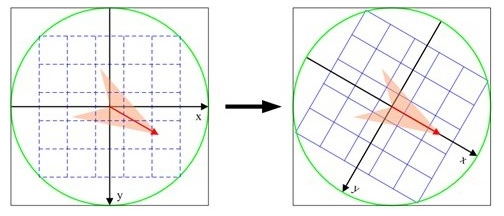
\includegraphics[width=0.5\linewidth]{yi}
\caption{将坐标移至关键点主方向}
\label{fig:yi}
\end{figure}
        
旋转后邻域内采样点的新坐标为:
\begin{align}
\left( \begin{array}{c}
x^{'} \\
y^{'} \\
\end{array} \right)
=\left( \begin{array}{cc}
\cos\sigma & -\sin\sigma \\
\sin\sigma & \cos\sigma \\
\end{array} \right)
\left( \begin{array}{c}
x \\
y \\
\end{array} \right)
\end{align}

下面就要对每个特征点求取方向直方图了,以特征点为原点,求其邻域内像素点的梯度方向直方图。梯度方向直方图是在$0\sim360$度的范围内,通常平均分为8等份,直方图中每一份是45度的范围。以特征点为中心,其周围$16\times16$的邻域内,计算每一个像素的梯度,看其梯度方向在哪一个度数范围内,直方图中就给相应的那一份加上一个权重,这里的权重就是每个像素梯度的大小。将$16\times16$的邻域再分为$4\times4$个区域,每个区域中有16个像素点,计算每个区域的梯度方向直方图,如图~\ref{fig: 128dimension}所示。这样对每个特征点就得到一个$4\times4\times8 = 128$维的特征描述子。
\begin{figure}
\centering
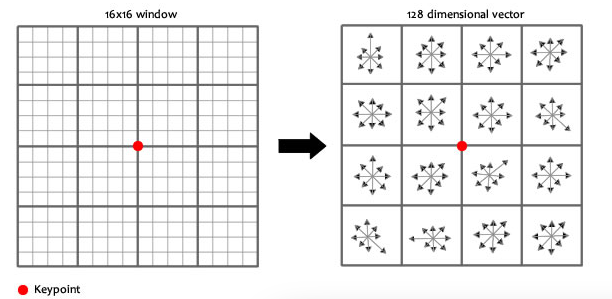
\includegraphics[width=0.5\linewidth]{sift2}
\caption{描述子用128维向量表征}
\label{fig: 128dimension}
\end{figure}

再以特征点为原点,求其邻域内像素点的梯度方向直方图。梯度方向直方图是在$0\sim360$度的范围内,通常平均分为8等份,直方图中每一份是45度的范围。假设邻域范围为$16\times16$,计算其中每一个像素的梯度,看其梯度方向在哪一个度数范围内,直方图中就给相应的那一份加上一个权重,这里的权重就是每个像素梯度的大小与高斯权重的乘积。

当邻域范围为$16\times16$时,我们通常将其又分为$4 \times 4$个区域,计算每一个区域中的8个方向的梯度方向直方图,即可形成一个种子点,一共可以生成16个种子点。

描述子向量元素门限化及门限化后的描述子向量规范化。

根据特征点的尺度对特征描述向量进行排序,生成最终的SIFT特征向量。
\end{enumerate}

\item 方向梯度直方图特征

方向梯度直方图~\cite{dalal2005histograms}(Histogram of Oriented Gradients,HOG)特征是由Navneet Dalal等人于2005年提出的一种特征描述子,它是一种局部特征,主要通过统计图像上局部区域内的梯度方向来构成直方图,最后将所有区域内的直方图串联而成。方向梯度直方图特征结合支持向量机分类算法生成分类器在图像识别方面取得了很好的效果,特别是在行人检测的应用中更是起到了重要作用。对方向梯度直方图进行求解的具体步骤如图~\ref{fig: shixian}。
\begin{figure}
\centering
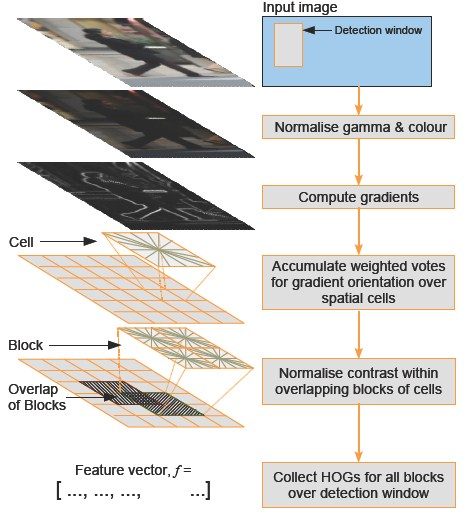
\includegraphics[width=0.4\linewidth]{flowchart}
\caption{HOG特征}
\label{fig: shixian}
\end{figure}

\begin{enumerate}
\item 首先对图像进行标准化或归一化操作。由于拍照光线不好、角度问题以及噪声等的影响,所得到的图像会有对比度低、局部昏暗等问题,对于随后的特征提取会有一定的干扰。通常采用Gamma校正法来对颜色空间进行标准化,Gamma压缩公式为:

\begin{align}
I(x,y)=I(x,y)^{gamma}
\end{align}

\item 利用一阶微分计算每一个像素的梯度(包括大小和方向),梯度方向同时也表示了目标物体的轮廓边界方向。
    
采用模板$[-1~0~1]$计算水平和垂直方向的梯度:
\begin{align}
G_{h}(x,y)=f(x+1,y)-f(x-1,y)~~~~\forall x,y\\
G_{v}(x,y)=f(x,y+1)-f(x,y-1)~~~~\forall x,y
\end{align}
        
梯度值和梯度方向的计算如下:
\begin{align}
M(x,y)=\sqrt{G_{h}(x,y)^{2}+G_{v}(x,y)^2}\\
\theta(x,y)=\arctan\frac{G_{h}(x,y)}{G_{v}(x,y)}
\end{align}
        
\item 将图像划分成小的单元(cell)(例如$6 \times 6$像素/单元)。

\item 统计每个单元内所有像素点的梯度直方图,将其作为每个单元的描述子。首先将梯度方向分为$m$份(共360度),如果分为了16份(如图~\ref{fig: bin}),则每一份中是22.5度。然后看每个像素点的梯度方向是落在了哪一份中,对应直方图中的那一份就加上一个权值,这里的权值就是像素点的梯度大小。
\begin{figure}
\centering
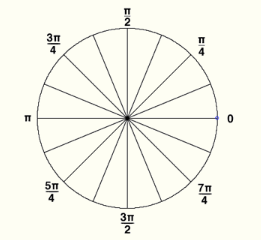
\includegraphics[width=0.3\linewidth]{bin}
\caption{梯度方向bin}
\label{fig: bin}
\end{figure}
       
\item 相邻的几个单元可以组成一个更大的块(block)(例如$3 \times 3 $个cell/block),再将一个块内所有单元的梯度直方图串联起来,最后得到该块的方向梯度直方图特征描述子。在将单元组合成块时,块与块之间是可以有重合的,这样,每个单元的梯度直方图都会被多次使用,以串联生成块的梯度直方图特征。其中块既可以按矩形划分(R-HOG),也可以按环形划分(C-HOG),具体见图~\ref{fig:shape}。
    
\begin{figure}
\centering
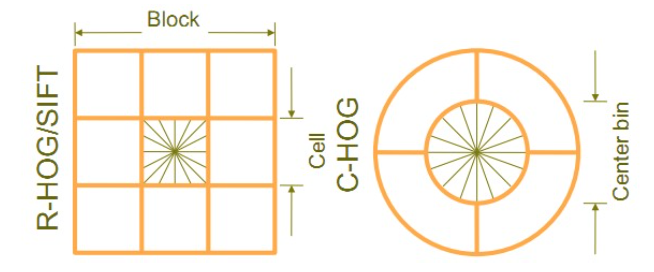
\includegraphics[width=0.5\linewidth]{shape}
\caption{矩形区间和环形区间}
\label{fig:shape}
\end{figure}
        
\item 将图像内的所有块的梯度方向直方图特征串联起来就可以得到整幅图像的梯度方向直方图特征描述子了,这个就是最终的可供分类使用的特征向量。该向量的维数为$m \times n \times \alpha$,其中$m$表示每个单元中方向bin的数目,$n$、$\alpha$分别表示块的个数以及一个块中的单元数目。
\end{enumerate}

\item SURF

SURF与SIFT算法相似,其优点是运算简单,效率高,缺点是不够稳定,并且检测出的特征点数目少一些。

算法步骤如下:

\begin{enumerate}
\item 构建Hessian矩阵。采用的是Hessian矩阵行列式近似值图像。

\item 构造多尺度空间。

构造对尺度空间的目的是实现尺度不变性,SURF算法则用高斯滤波与Hessian矩阵结合近似实现多尺度空间,计算复杂度比SIFT低。

\item 根据非极大值抑制初步确定特征点。

\item 主方向确定

\item 构造特征点算术描述子,SURF算法是选取一个20S(单位)的区域,分成$4 \times 4$分,每一份中有$5 \times 5$S,统计一份中的$\sum d_{x}$,$\sum d_{y}$,$\sum |d_{x}|$,$\sum |d_{y}|$,这样就得到$4 \times 4 \times 4 = 64$的向量描述子。SIFT是128个描述子,比SURF复杂一点。
\end{enumerate}

\item 局部二值模式特征

局部二值模式(Local Binary Pattern,LBP)~\cite{ojala1994performance}是一种用来表征图像局部纹理特征的描述子,具有旋转不变性和灰度不变性等优点。
 
 对图像中的某个像素点计算其局部二值模式值的步骤如下:以该像素点为中心,将其灰度值与其周围$3\times3$窗口的邻域内的8个像素点进行大小比较,如果邻域内像素的灰度值大于中心点的灰度值,则该邻域内像素点的值被置为1,否则置为0。经过这一阈值处理后,对每一个像素点,就得到了其邻域8个像素点的二进制表示(方向是从左上方的像素点开始往右顺时针走),再求出该二进制数的十进制表示,这就是该中心像素点上的局部二值模式值,如图~\ref{fig: lbp}。
\begin{figure}[!ht]
\centering
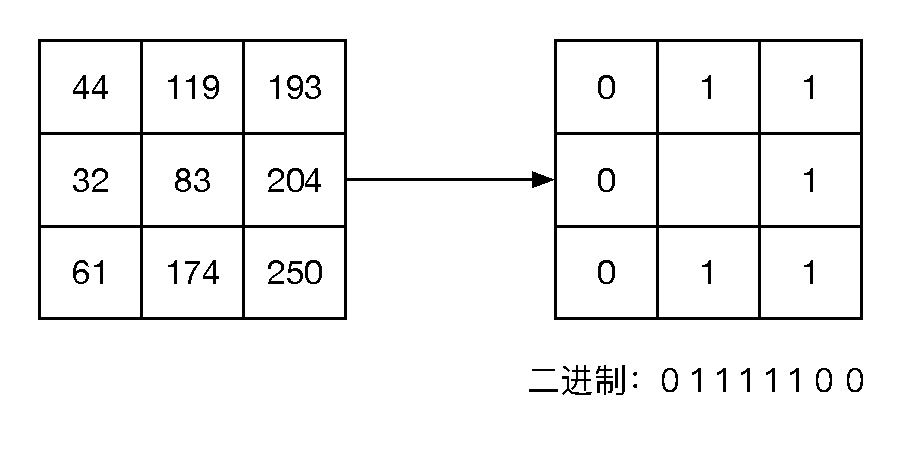
\includegraphics[width=4in]{lbpbinary.eps}
\caption{LBP特征}
\label{fig: lbp}
\end{figure}

\item FV(Fisher vector)
   
Fisher vector本质上是用似然函数的梯度vector来表达一幅图像。主要思路是用生成式模型(GMM)对样本输入进行建模,进而得到样本的一种表示(fisher vector),再将这种表示(fisher vector)输入判别式分类器(SVM)得到图像分类结果。fisher vector是fisher kernel中对样本特征的一种表示,它把一幅图片表示成一个向量。在高斯分布的基础上再找到变化的方向,可以更加准确的表示这一张图。

\item 骨架特征

骨架又称为中轴,它的定义来自于烧草模型和最大圆盘模型。骨架不仅包含了物体的几何特征,也描述了物体的拓扑结构。经典的骨架化算法有中轴变换、细化算法、Voronoi图算法等。在骨架的基础上可以通过奇点图、骨架树等对物体的结构特征进行描述。

骨架树:将骨架映射到一个树状结构(如图~\ref{fig: skeleton-tree})。骨架上的点可以分为三种类别:分叉点、端点和连接点。其中当骨架点的邻接点的数目为1时被称为端点,邻接点数目为2个或2个以上时被称为分叉点,除此之外的点被称为连接点。
\begin{figure}
\centering
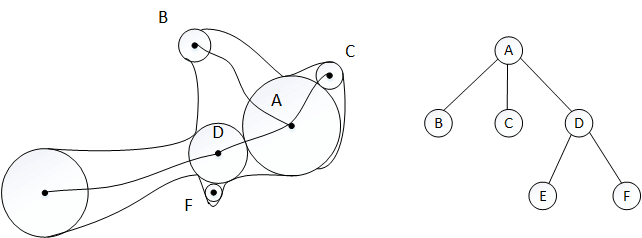
\includegraphics[width=0.6\linewidth]{skeleton-tree.png}
\caption{骨架树}
\label{fig: skeleton-tree}
\end{figure}
根据骨架树深度优先搜索产生的节点序列中的所有节点用其孩子数替换,替换后得到的新序列即为树描述符。例如,图~\ref{fig: skeleton-tree}的树描述符为(3,2,0,0,0,0)。

\item 形状上下文特征
    
    形状上下文(Shape Context, SC)由Belongie等人~\cite{belongie2002shape}提出,是基于物体轮廓样本点进行描述的。下面给出形状上下文求解的具体步骤。
    首先,对一幅图像(图~\ref{fig: ShapeDescription}(a))中的目标进行边缘提取,得到结果如图~\ref{fig: ShapeDescription}(b)所示。然后将这一轮廓看作是一定数目的采样点的集合(图~\ref{fig: ShapeDescription}(c)),利用这些采样点来描述目标形状。通过对数极坐标空间(图\ref{fig: ShapeHistogram}(a))计算每个采样点与形状其他点之间的位置关系,采用直方图表示。假设目标轮廓上采样点的集合定义为$O = \{o_1, \ldots, o_n\}$,其中$n$表示采样点的个数。假设目标轮廓是分段平滑的,当$n$充分大时,可以基本与物体实际轮廓贴合。若第$i$个采样点$o_i$作为参考坐标原点(图~\ref{fig: ShapeHistogram}(b)),建立对数极坐标映射表示剩余的$n-1$个采样点的分布情况,可以看到周围与它相邻的点(在极坐标覆盖的范围之内)落于不同的小格子内,表示不同的相对向量,这些相对向量刻画了整个形状与参考点的相对位置,因而就成为这个点的形状上下文,用直方图$h_i$表示。
\begin{align}
h_i(k) = \# \{j \ne i : (o_j - o_i) \in bin(k)\}
\label{eq: shape context}
\end{align}
以$o_i$为极坐标中心进行坐标变换,以该中心画一个圆,并把圆等分成$k$份,计算圆范围内的点落在每一份中的个数,这样对每一个点就得到一个$k$维的直方图。$\theta$为极角,$r$为极坐标半径,对于每一个由$\theta$和$logr$确定的极坐标区域,如果该区域包含的点越多,那么在由$\theta$和$logr$确定的对应形状直方图中的数值就越大。 

\begin{figure}[t]
  \centering%
  \begin{subfigure}{0.23\linewidth}
    
\includegraphics[height=3.5cm]{a1.png}
    \caption{}
  \end{subfigure}
 % \hspace{4em}%
  \begin{subfigure}{0.23\linewidth}
    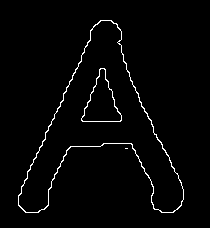
\includegraphics[height=3.5cm]{a-edge.png}
    \caption{}
  \end{subfigure}
   \begin{subfigure}{0.234\linewidth}
    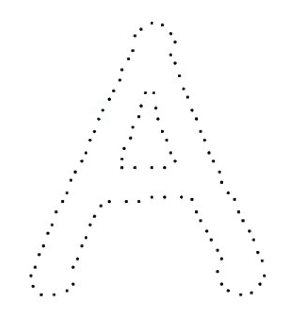
\includegraphics[height=3.5cm]{a-point.png}
    \caption{}
  \end{subfigure}
  \caption{形状描述}
  \label{fig: ShapeDescription}
\end{figure}

\begin{figure}[t]
  \centering%
  \begin{subfigure}{0.3\linewidth}
    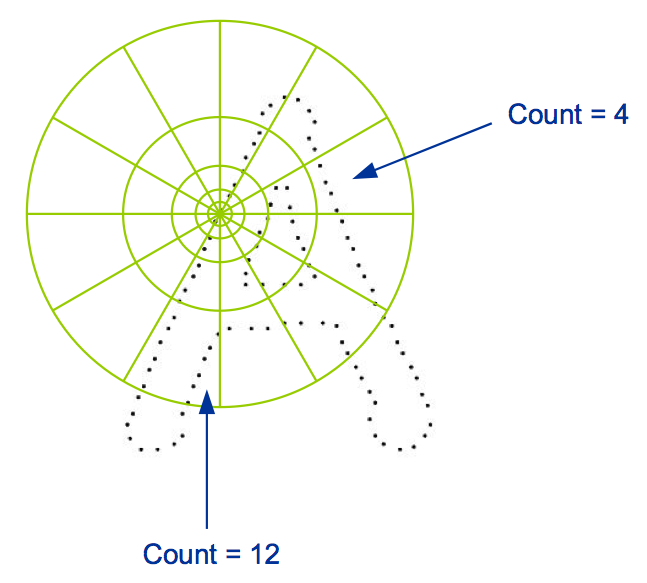
\includegraphics[height=4cm]{a-log.png}
    \caption{}
  \end{subfigure}
  \hspace{4em}%
  \begin{subfigure}{0.35\linewidth}
    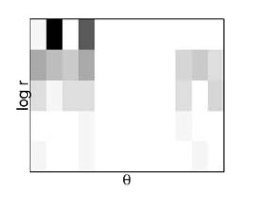
\includegraphics[height=4cm]{his.png}
    \caption{}
  \end{subfigure}
  \caption{形状上下文的直方图表示}
  \label{fig: ShapeHistogram}
\end{figure}


只要每个点的形状上下文出来了,那么对所有点的形状上下文组合起来就可以形成整个物体的形状上下文了。

在物体分类识别的应用中,是这样利用形状上下文特征的:首先对图像数据集中的每一类别都找一幅模板图像,该模板能较好地反应其所属类别图像的共性。假设对一幅图像的物体轮廓采样了100个点,就得到一个$100\times k$的矩阵。同样,对模板也能得到一个$100\times k$的矩阵。再计算图像中的每个点与模板中的每个点的距离,得到图像中的点和模板中的点的一一对应关系,结果是一个$100\times100$的矩阵。最后根据这个一一对应关系计算出一个值,表示该图像和模板之间的相似度。计算出每幅图像和所有类别模板之间的相似度,当做该幅图像的一个特征向量,利用分类算法进行训练,可以生成一个分类器。
\end{enumerate}

\subsection{其它特征}

\begin{enumerate}

\item 局部对称性

\begin{figure}[!ht]
 \centering
 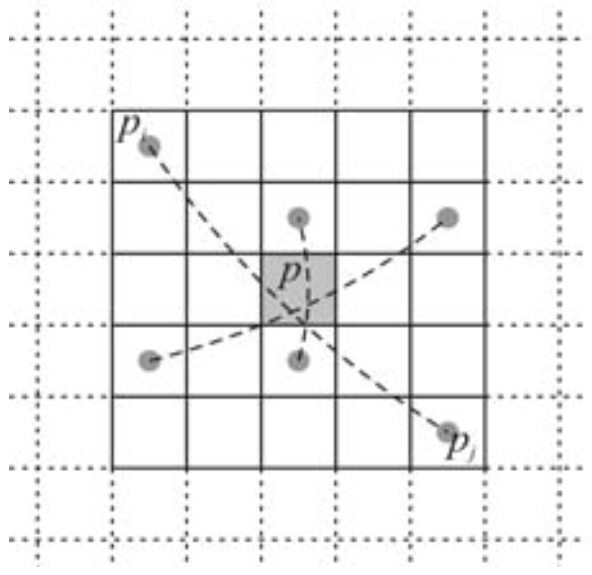
\includegraphics[width=3in]{ExamplesofPixelpairs}
\caption{用对称性算子来对像素对的梯度进行比较的三个例子}
\label{fig: ExamplesofPixelpairs}
\end{figure}

局部对称性的原理是基于周围像素的灰度梯度,计算在给定点$p$处的对称性程度。如图~\ref{fig: ExamplesofPixelpairs}所示,点$p$处的对称性可以通过比较位于$p_i$和$p_j$处的像素对$i$和$j$的灰度梯度来度量,其中$p = (p_i  = p_j)/2$。每对像素对对点$p$处的局部对称性的贡献为
\begin{align}
c(i, j) = d(i, j, \sigma) \cdot p(i, j) \cdot m_i \cdot m_j
\end{align}
$m_i$是像素点$i$的梯度的模,$d(i, j, \sigma)$是当标准差为$\sigma$时,两个像素点间的距离的高斯加权函数,对称性
\begin{align}
p(i, j) = \Big(1-cos(\gamma_i+\gamma_j)\Big)\cdot \Big(1-cos(\gamma_i-\gamma_j)\Big)
\label{eq: SymmetryMeasurement}
\end{align}

其中,$\gamma_i = \theta_i-\alpha$,见图~\ref{fig: PixelpairContribution}。当点$p_i$、$p_j$关于点$p$对称时,$\gamma_i+\gamma_i=\pi$,式~(\ref{eq: SymmetryMeasurement})中的第一项取得最大值。如果只用第一项,会使得在直线边缘上的点取得较大的值,而这些点通常并不具有对称性。为了避免这个问题,又加入了第二项,表示具有相似梯度方向的像素对。最后,对所有像素对的贡献进行求和得到点$p$处的isotropic symmetry值
\begin{align}
M^{iso}(x, y) = \sum_{(i, j)\in \Gamma(p)} c(i, j)
\label{eq: IsotropicSymmetry}
\end{align}

\begin{figure}[!ht]
 \centering
 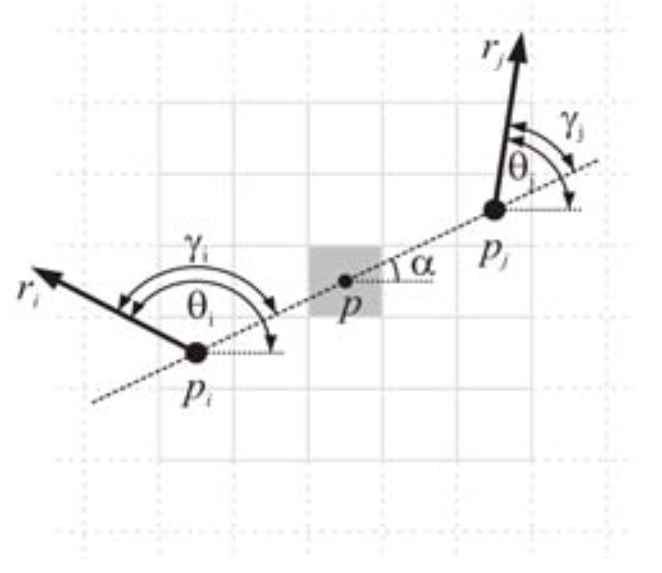
\includegraphics[width=3in]{PixelpairContribution}
\caption{每对像素对的贡献的几何表示}
\label{fig: PixelpairContribution}
\end{figure}

为了使symmetry operator对有多个对称轴的对称图案更敏感,Reisfeld等人~\cite{reisfeld1995context}又提出了radial symmetry operator,作为isotropic symmetry operator的扩展。首先,像素对的贡献的方向用$\varphi(i, j) = (\theta_i+\theta_j)/2$来计算。然后,对最大贡献为$c(i, j)$的像素对$(i, j)$,对称方向被确定为$\phi(p) = \varphi(i, j)$。这个值也用来提升有不相似方向的像素对的贡献。
\begin{align}
M^{rad}= \sum_{(i, j)\in \Gamma(p)} c(i, j) \cdot sin^2(\varphi(i, j) - \phi(p))
\end{align}

\item 灰度直方图

灰度直方图是针对灰度图像的,如果是彩色图像,可以求取其颜色直方图。若灰度级的范围为$0 \sim 255$,则灰度直方图表示这256个灰度值中的每一个在图像中出现的个数。
\end{enumerate}

\section{特征选择}

~\ref{2.3.3}和~\ref{3.1}节的介绍中基本涵盖了近年来图像处理和机器视觉领域常用的一些特征,其中有些特征适用于浮游动物图像的分类问题,有些并不适用,要对这些特征进行筛选。本文中的特征选择过程是通过对单个特征及特征组合的理论分析与实验结合,判断一个特征或一组特征对浮游动物图像分类效果的影响。其中实验部分是对~\ref{2.1}节中介绍的包含13类浮游动物的数据集分别用两种基本的分类算法(支持向量机和随机森林)进行分类,对分类结果利用$K$折交叉验证方法进行评价,看在数据集上的分类准确率和错误率有没有分别提高和降低。

对前面所总结的所有特征进行实验,我们最终选择了三类特征:PkID中用到的特征、LBP特征以及内距离形状上下文特征。相对于其它特征而言,这三类特征在对浮游动物图像的分类上效果较好,其中PkID中用到的特征数目较多,可对其进行进一步筛选。

\subsection{PkID中的22个特征}

由~\ref{2.3.3}节可以看到,PkID中共采用了67个特征,分为6大类:位置特征、尺寸特征、灰度特征、形状特征、生物统计特征和自定义特征。这些特征都是带有一定意义的,通过实验和分析,我们得出结论:位置特征不能表征浮游动物的属性,会降低分类准确率。而由于我们采用的数据集是经过扫描得到的,不同浮游动物类别有透明和不透明之分,表现在扫描图像上就是灰度值高和灰度值低,因而灰度特征可作为浮游动物图像分类的一个重要特征。由于数据集中对每幅图像都做了标尺,不同类别的浮游动物在尺寸上应该是互不相同的,但由于处于不同成长期的浮游动物以及拍摄角度(正面和侧面)的影响,会使得尺寸特征失去了本应有的效果。形状特征是表征一类物体的较为重要的特征,对于不同种类有一定的区分度。生物统计特征近年来在分类识别中使用的也比较多,效果较好,但其物理意义不是十分明确,难以从理论上说明其有用的原因,只能从实验结果上反应。

\begin{table}[ht]
\centering
\caption{对PkID中的6类特征用支持向量机和随机森林方法进行分类的分类准确率}
\begin{tabular}{|c|c|c|}
\hline
& 支持向量机 & 随机森林 \\
\hline
位置特征 & 15.3\% & 30.23\% \\
\hline
尺寸特征 & 26.04\% & 56.95\% \\
\hline
灰度特征 & 37.6\% & 61.3\% \\
\hline
形状特征 & 37\% & 63.1\% \\
\hline
生物统计特征 & 52.4\% & 69.9\% \\ 
\hline
自定义特征 & 68.05\% & 69.03\% \\
\hline
\end{tabular}
\label{PkID-6}
\end{table}

我们对这6类特征分别用支持向量机和随机森林分类算法进行实验,得到的分类准确率如表~\ref{PkID-6}所示。效果比较好的是灰度特征、形状特征、生物统计特征和自定义特征,基本符合我们对于特征的分析,从而可以将位置特征和尺寸特征筛除掉。对剩下的4类特征进行进一步实验,不断地挑选一定数量的特征,用支持向量机和随机森林分类算法进行验证,最终我们从67个PkID特征中挑出了22个,如表~\ref{表2}所示,可以看到只选取了生物统计特征、形状特征、自定义特征三种,其中一部分自定义特征是根据其他几类特征来自定义产生的,所以这里没有选取灰度特征,分类效果依然很好。

\begin{table}[htbp]
\centering
\caption{PkID中的22个特征}
\begin{tabular}{|c|l|}
\hline
生物统计特征 & Mean、StdDev、Skew、Kurt、CV、SR \\
\hline
形状特征 & Fractal、Skelarea、Circ、Symetrieh、Symetriev、Symetriehc、\\
 & Symetrievc、Elongation2、Circexc、Convperim、Convarea\\ 
 \hline
自定义特征 & MeanPos、PerimAreaexc、FeretAreaexc、PerimFeret、CDexc \\
\hline
\end{tabular}
\label{表2}
\end{table}

\subsection{局部二值模式}

   
对LBP特征向量进行提取的步骤:
\begin{enumerate}
    \item 首先将检测窗口划分为$16\times16$的单元(cell)。
    \item 对于每个单元中的一个像素,将相邻的8个像素的灰度值与其进行比较,若周围像素值大于中心像素值,则该像素点的位置被标记为1,否则为0。这样,$3\times3$邻域内的8个点经比较可产生8位二进制数,即得到该窗口中心像素点的LBP值。
    \item 然后计算每个单元的LBP值直方图,即每个数字(假定是十进制数LBP值)出现的频率,然后对该直方图进行归一化处理。
    \item 最后将得到的每个单元的统计直方图进行连接成为一个特征向量,也就是整幅图的LBP纹理特征向量。
\end{enumerate}

\subsection{内距离形状上下文}

本文~\ref{2.3.2}节中介绍了关于形状上下文的内容,由于形状上下文不能很好地解决物体类内部之间的变形,后期产生了改进的基于内部距离的形状上下文~\cite{ling2007shape},内距离形状上下文中采用内距离代替欧式距离。

采用内距离形状上下文提取图像特征的基本步骤如下:
\begin{enumerate}
\item 先从图像中挑选$m\times n$张图像作为模板(每类浮游动物中选取$m$张,共$n$类)。
\item 采用内距离形状上下文分别计算训练集和测试集中所有图像和上一步骤中$m\times n$张图像间的距离。
\item 将上面计算得到的距离矩阵作为训练集和测试集的特征,输入到ELM中进行学习和分类。
\end{enumerate}

\chapter{分类器设计}

\section{常用的分类技术}
\label{4.1}

\subsection{支持向量机方法}

支持向量机(Support Vector Machine,SVM)~\cite{cortes1995support}是一种有监督的统计学习方法,能够最小化经验误差和最大化几何边缘,被称为最大间隔分类器,可用于分类与回归分析。SVM的基本原理是在高维空间中寻找一个分类超平面,将不同类别的数据样本点分开,使不同类别的点之间的间隔最大,该分类超平面即为最大间隔超平面,对应的分类器称为最大间隔分类器。针对二分类问题,图~\ref{fig: svm}可以直观地描述SVM的空间特征。

\begin{figure}[!ht]
 \centering
 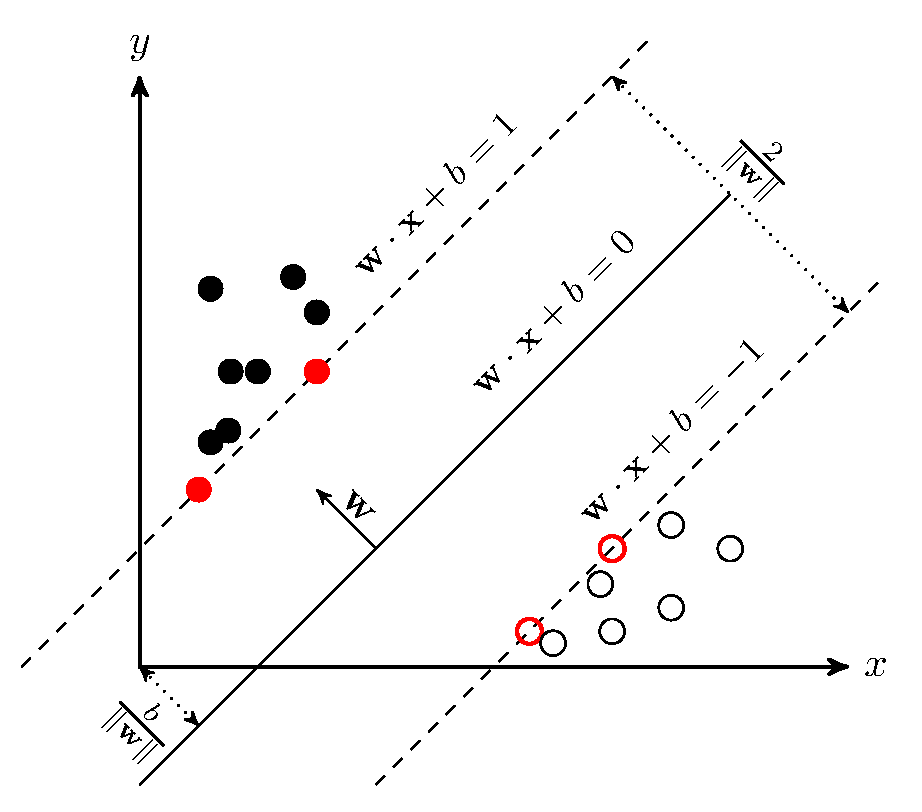
\includegraphics[width=4in]{svm.png}
\caption{SVM的训练数据样本及空间特征}
\label{fig: svm}
\end{figure}

假设数据样本为$x_1, x_2, \ldots, x_n$,分类超平面可以表达为:
\begin{equation}
w_Tx - b = 0 
\end{equation}

其中,$x$为分类超平面上的点;$w$为垂直于分类超平面的向量;$b$为位移量,用于改善分类超平面的灵活性,超平面不用必须通过原点。

两个分类超平面之间具有最大间隔,需要知道训练样本中的支撑向量、距离支撑向量最近的平行超平面,这些平行超平面可以表示为:
\begin{align}
\left\{ \begin{array}{l}
w^T x - b = 1\\
w^T x - b = -1
\end{array} \right.
\end{align}

其中,$w$是分类超平面的法向量,长度未定;1和-1只是为了计算方便而取的常量,其他常量只要互为相反数亦可。

如果给定的训练样本是线性可分的,那么就可以找到两个间距最大的平行超平面,并且这两个超平面之间没有任何训练样本,它们之间的距离为$2/||w||^2$。所以最小化$||w||^2$,就可以使这两个超平面之间的间隔最大化。
\begin{align}
min \; \frac{1}{2}||w||^2\\
s.t.\; y_i(w^Tx_i + b) \ge 1
\end{align}

通过将目标函数转化,求解SVM可以变成一个标准的凸优化问题。因为目标函数是二次的,而约束条件是线性的,所以这是一个凸二次规划问题。虽然这个问题是一个标准的二次规划问题,但同时具有它的特殊结构,通过将此二次规划问题转化为其对偶问题,可以找到更加有效的方法进行求解。整个对偶问题可表示为:
\begin{align}
\max_a\sum_{i = 1}^n\alpha_i - \frac{1}{2}\sum_{i, j = 1}^n\alpha_i\alpha_j y_i y_j < x_i \cdot x_j >\\
s.t. \; 0 \le \alpha_i \le C, i = 1, \ldots, n \\
\sum_{i =1}^n\alpha_i y_i = 0
\end{align}
其中,$\alpha$为引入的拉格朗日乘子。经计算,最优权值向量$w^*$和最优偏置$b^*$分别为
\begin{align}
w^* = \sum_{i= 1}^n \alpha_i^*y_i x_i \\
b^* = y_i - \sum_{i = 1}^n y_i \alpha_i^*(x_i \cdot x_j)
\end{align}
其中,$i\in \{ i|\alpha_i^* > 0\}$。因此得到最优分类面$(w^* \cdot x) + b^* = 0$,而最优分类函数为
\begin{align}
f(x) = sgn\{(w^* \cdot x) + b^*\} = sgn\{(\sum_{i = 1}^n\alpha_i^*y_i(x_i \cdot x_j)) + b^*\}
\end{align}

\subsection{随机森林方法}

在介绍随机森林方法之前,首先介绍决策树的概念,决策树是一种树,树中每个节点用于表示某个对象,每个分叉路径用于代表某个可能的属性值,从根节点到某叶节点所经历的路径所表示的对象值则对应该叶节点。

为了提高识别精度,必须要通过某种衡量准则选择特征,使得分割后的数据集的标签信息增益最大。信息增益是用于衡量给定属性区分训练样本能力的度量值,它的求解是用原始数据集标签熵减去分割后的数据集标签熵,如果熵变小了,则信息增益变大,表示给定属性对数据集的分类带来了一定的信息量。熵是信息论中广泛使用的一个度量标准,用于表示一件事情的不确定性,当要搞明白一件事所要求的信息量越高,这件事的不确定性越大,因而熵越大。假设$S$是包含关于某个目标概念的样本集,目标属性具有$m$个不同的种类,那么$S$相对于这$m$个状态类别的熵定义为:
\begin{align}
Entropy(S) = \sum_{i = 1}^m -p_i log_2 p_i
\end{align}
其中,$p_i$为$S$中不同类别样本的比例。

一个属性的信息增益可以看作由于使用这个属性分割样本从而导致的期望熵降低,一个属性$A$相对样本集合$S$的信息增益$Gain(S, A)$计算公式为:
\begin{align}
Gain(S, A) = Entropy(S) - \sum_{v\in V(A)} \frac{|S_v|}{|S|} Entropy(S_v)
\end{align}
其中,$V(A)$是属性$A$的值域,$S$是样本集合,$S_v$是$S$在属性$A$上值等于$v$的样本集合。

整个处理流程如下:首先计算每个属性的信息增益,然后依照信息增益最大原则选取属性,作为分割样本的属性。接着构建决策树,采用递归思想依次分割下去,直到执行完成就构建好了决策树。最后依据决策树进行分类,给出序列化决策树。

随机森林是一种采用决策树作为作为基预测器的集成学习方法,2001年由Breiman提出~\cite{breiman2001random},通过自助重采样技术,从总数量为$N$的原始训练样本集中有放回地重复随机选取$N$个样本,由此得到一个自助训练数据集,按此方法重复得到一组自助训练数据集。对每个自助训练集,用决策树学习方法(如C4.5、ID3、CART算法)创建一颗完全生长的无剪枝处理的决策树,进而得到一组决策树的集合。

对每个节点按固定概率分布来随机选择数目固定为$m$的特征(假设训练样本的总特征数目为$M$,$m << M$),作为在该节点寻找最佳分裂的依据。在预测时,根据所有决策树对新数据预测结果的平均值或根据投票多少来决定。

\subsection{极限学习机方法}

极限学习机(Extreme Learning Machine, ELM)是一种新型神经网络算法,最早是由新加坡南洋理工大学的黄广斌教授于2004年提出来的~\cite{huang2004extreme}。极限学习机的前身是单隐藏层反馈神经网络,在此基础上加上了一种新型的快速学习算法,使得学习速度得到了很大程度的提高。

神经网络的最小单位为“神经元”,一个最简单的神经网络可以仅仅由一个“神经元”组成,如图~\ref{fig: neuron}所示。

\begin{figure}
\centering
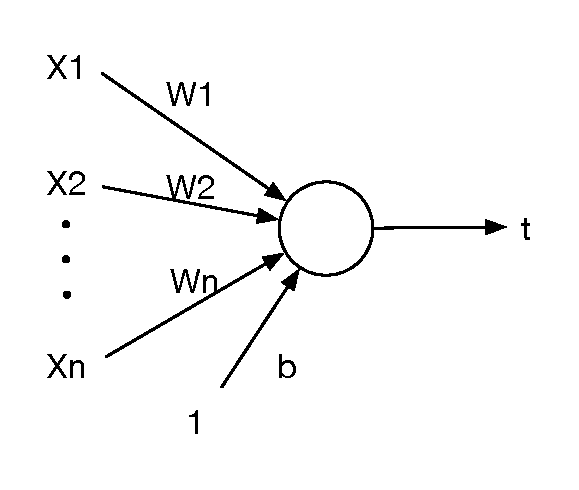
\includegraphics[width=0.3\linewidth]{neuron.eps}
\caption{单隐藏层反馈神经网络}
\label{fig: neuron}
\end{figure}

其中,第一列为输入向量,“1”表示截距,$b$表示偏置,箭头上的w为买个输入向量分量对应的权重值,最右端为输出。其输入-输出关系用数学公式表示为$y = g(w \cdot x + b)$,其中函数$g$叫做“激励函数”,通常采用sigmoid函数或tanh函数,这两个函数的表达式分别如下:
\begin{align}
g(z) = \frac{1}{1+exp(-z)}\\
g(z) = \frac{e^z - e^{-z}}{e^z + e^{-z}}
\end{align}
它们对应的图像分布见图~\ref{fig: sigmoid_tanh}。

\begin{figure}
\centering
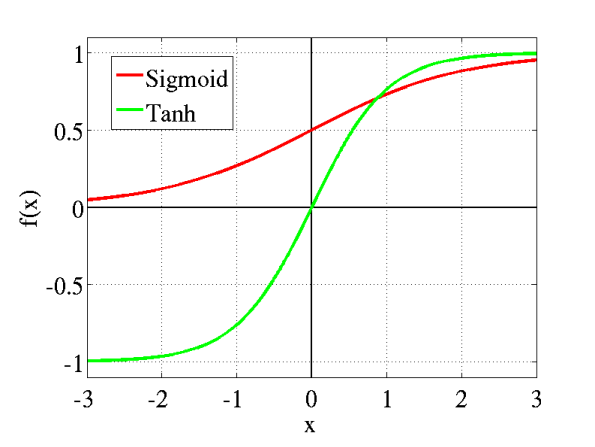
\includegraphics[width=0.5\linewidth]{sigmoid_tanh.png}
\caption{sigmoid和tanh函数的图像}
\label{fig: sigmoid_tanh}
\end{figure}

可以看出,这两个函数都是逻辑函数,因而这里的输入-输出关系是一种逻辑回归。

稍微复杂一点的神经网络是联结不只一个的神经元,常见的三层神经网络(单隐藏层反馈神经网络)如图~\ref{fig: ELM-network}所示。

\begin{figure}
\centering
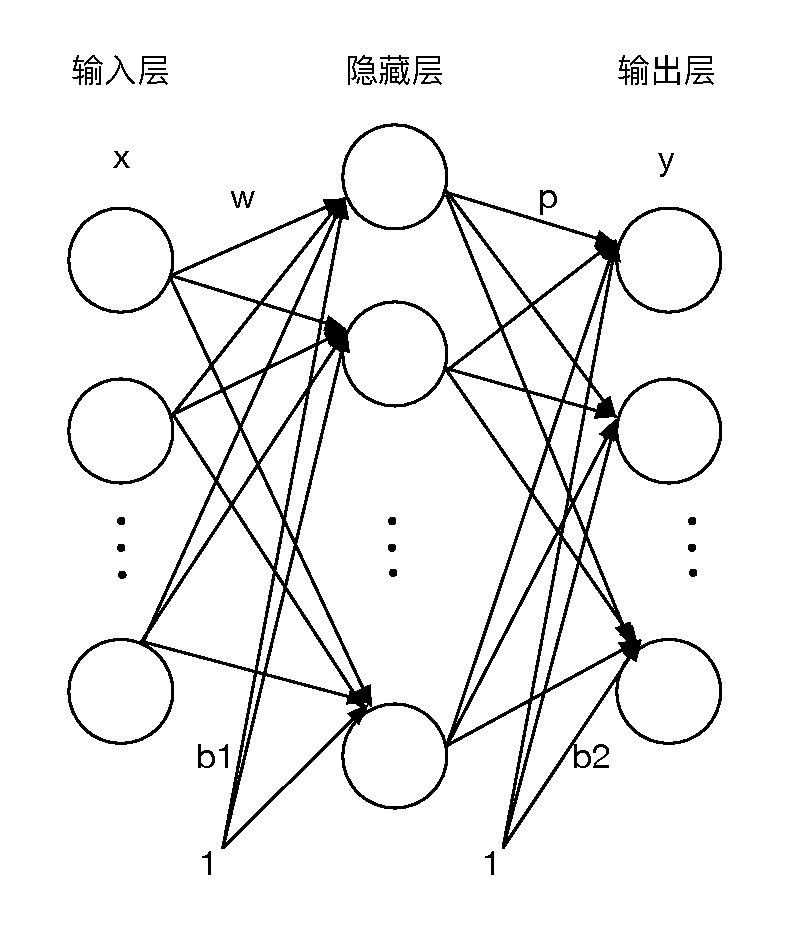
\includegraphics[width=0.5\linewidth]{Neural-network.eps}
\caption{单隐藏层反馈神经网络}
\label{fig: Neural-network}
\end{figure}

其中最左边一层叫做输入层,中间的一层叫做隐藏层,最右边一层叫做输出层。只有输入层和输出层可以跟外界进行联系,而隐藏层中的内容就对应一个黑盒子,外界无法观测到其值。从左往右来看,左边一层的输出总是连接着右边一层的输入,因而输出层第$k$个神经元的响应可以表示为:
\begin{align}
y[k] = [g(w_1 \cdot x + b_1) \cdot g(w_2 \cdot x + b_2) \cdot \ldots \cdot g(w_L \cdot x + b_L)] \cdot p_k + b_2[k], \; k = 1, \ldots, m
\end{align}
其中,$w_i$是一个向量,表示隐藏层第$i$个神经元的输入权重,$p_i$也是一个向量,表示输出层第$k$个神经元的输入权重。

单隐藏层反馈神经网络的主要优点为:1)可以充分拟合出任何复杂的输入-输出关系;2)每一层中单个的神经元以及一条连接对整个神经网络的作用是很小的,当少量神经元和连接发生错误时,对整个网络的影响不大,这样就增强了网络的容错性。其缺点是学习速度较慢,在时间消耗上远高于我们所能接受的最多时间。为了解决这一问题,很多研究者对单隐藏层反馈神经网络进行了进一步的探索,从而在运行时间上有了改进。

黄广斌教授通过对单隐藏层反馈神经网络的进一步研究发现,当“激励函数”$g$能够在任何一个区间内都满足无限可微的条件时,我们就可以随机地生成$w_i$和$b_i$的值,不用对它们进一步调整了。并且 在某种情况下$||T - Hp||_F = 0$一式是成立的,因而输出层的偏置也就可以忽略了。这样就可以得到一个新的单隐藏层反馈神经网络,叫做极限学习机网络,如图~\ref{fig: ELM-network}所示。
\begin{figure}
\centering
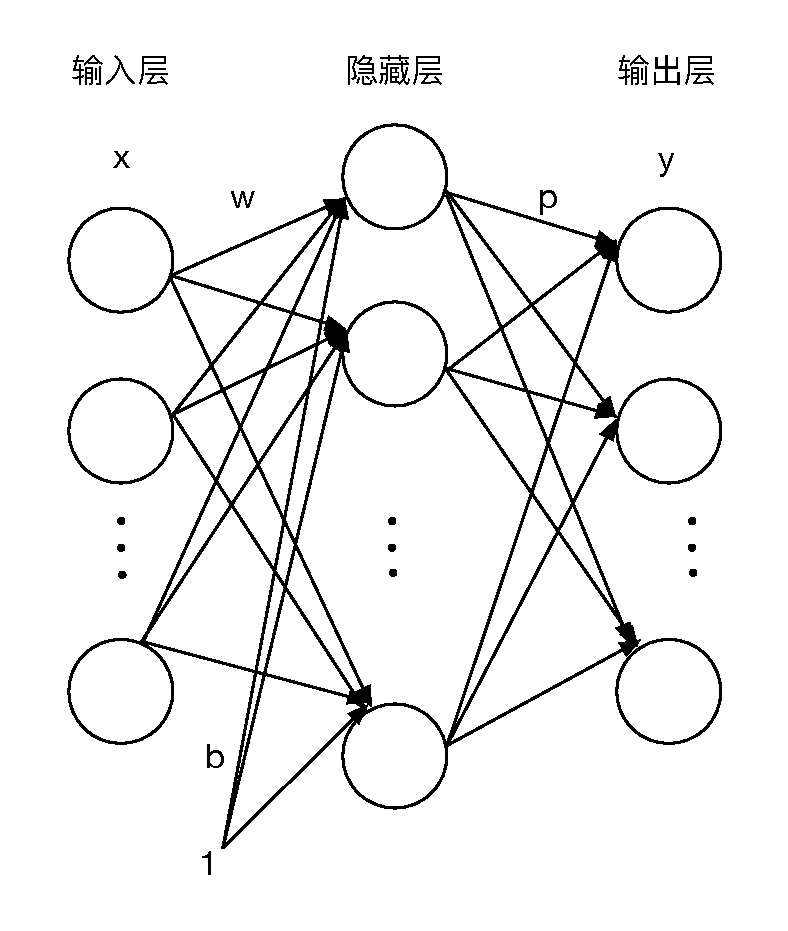
\includegraphics[width=0.5\linewidth]{ELM-network.eps}
\caption{极限学习机网络}
\label{fig: ELM-network}
\end{figure}

与单隐藏层反馈神经网络相比,极限学习机具有以下几个优点:
\begin{enumerate}
\item 忽略了输出层偏置,并且通过随机的方式产生隐藏层的偏置和输入层的权重,需要计算的就只剩下输出层的权重了。比单隐藏反馈网络要求解的内容少了很多,因而学习时间大大降低。在实际实验中,采用极限学习机算法进行训练通常几秒就完成了,而用单隐藏层神经网络进行训练往往需要几十甚至几百倍的时间。
\item 泛化能力更强。
\item 避免了所求解的局部最优问题以及过拟合的问题。
\end{enumerate}

\section{分类算法选择}

目前分类算法有很多种,而对于挑选出来的三类特征,我们将通过具体实验来选出适用每一类特征的分类算法。从论文~\cite{gorsky2010digital}中,我们知道对PkID中的特征,采用随机森林分类算法的分类准确率最高,因而对于我们挑选出的PkID中的22个特征,随机森林算法也应该最适用。在图像处理和机器视觉领域,LBP特征一般使用支持向量机分类算法进行分类,内距离形状上下文一般使用极限学习机进行分类。下面通过具体实验来进行验证,对这三类特征分别用~\ref{4.1}节介绍的三种分类进行分类,从而选出其最适用的分类算法。

首先对于PkID中的22个特征用支持向量机、随机森林、极限学习机分类算法分别进行分类,对分类结果用$K$折交叉验证进行评价,结果是用随机森林算法分类效果最好,结果如表~\ref{22-Features-RF}所示,分类准确率达到73\%,错误率为21.9\%。

\begin{table}
\centering
\caption{PkID的22个特征采用随机森林进行分类的结果}
\begin{tabular}{c}
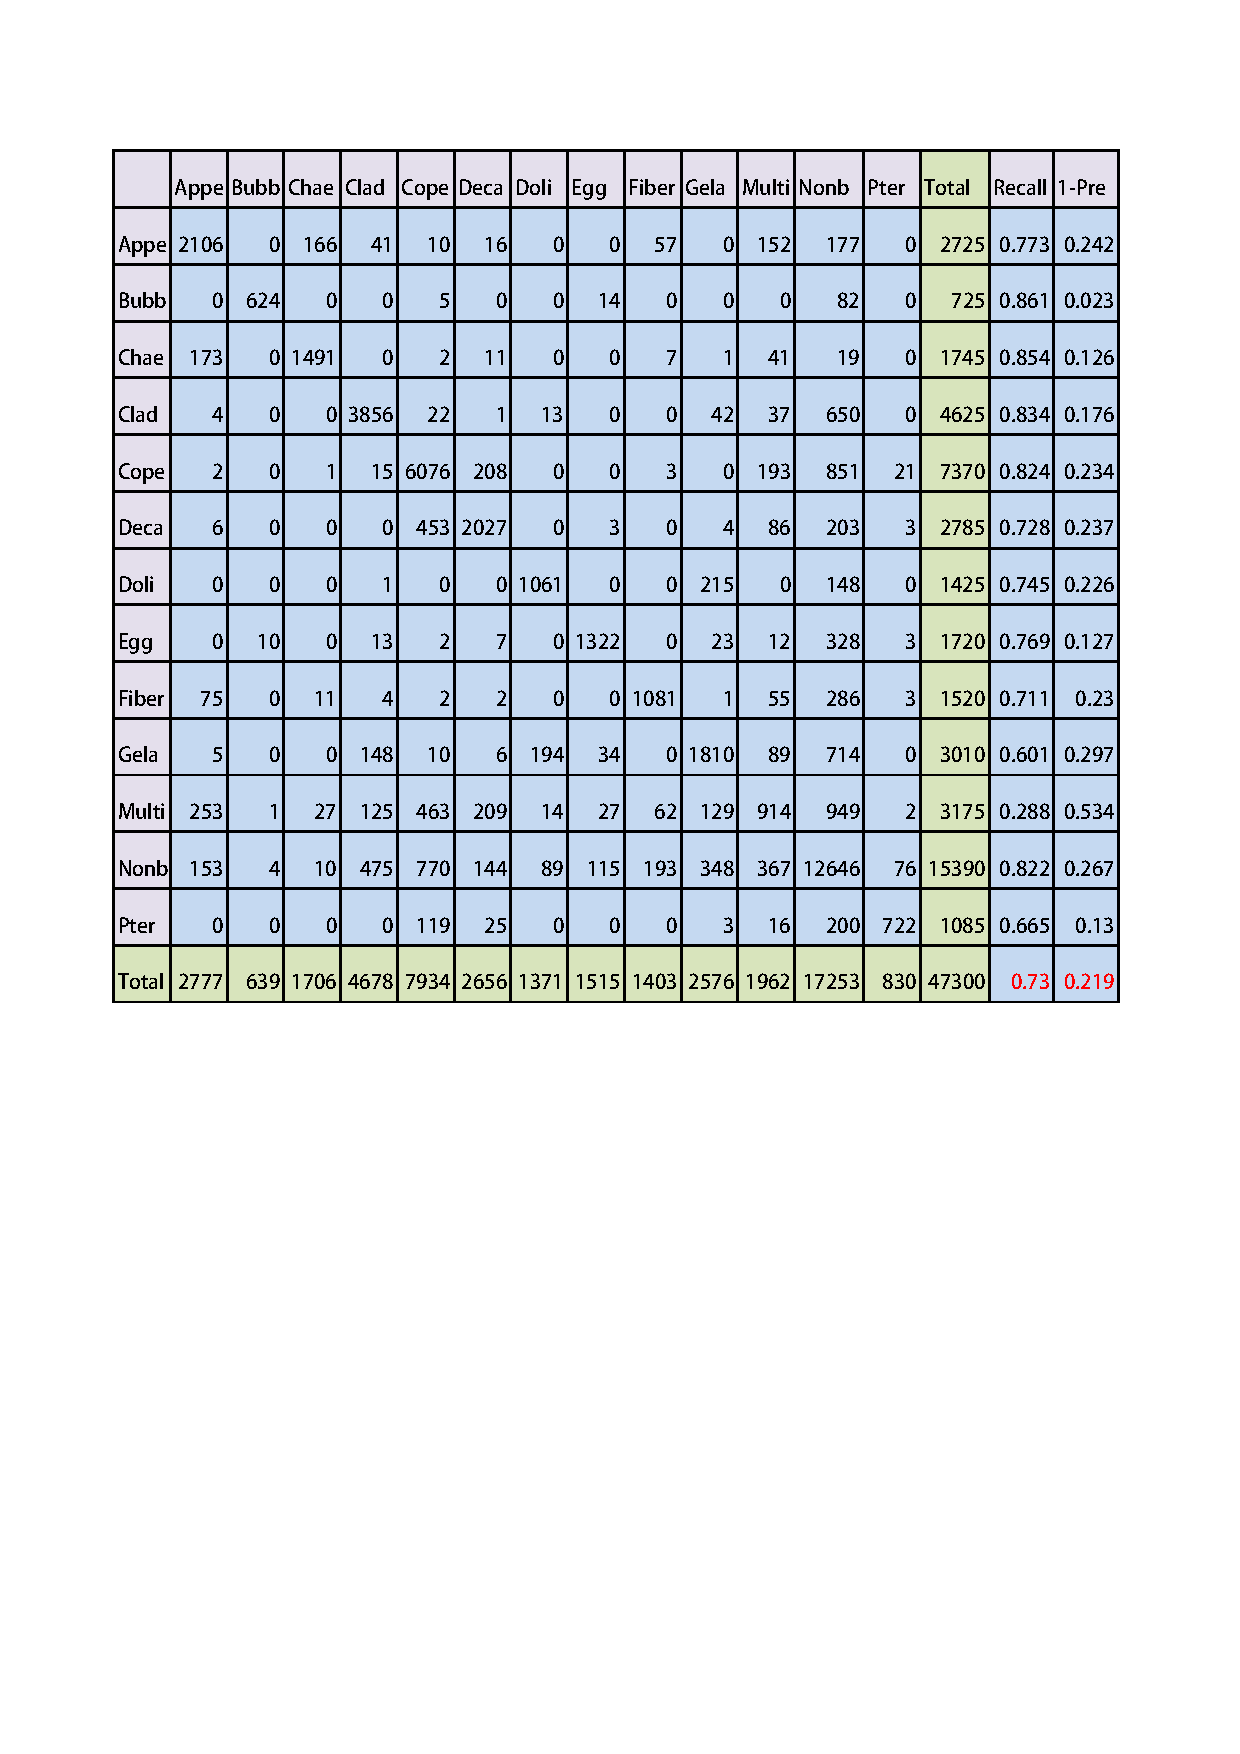
\includegraphics[width=1.0\linewidth]{22-Features-RF.pdf}
\end{tabular}
\label{22-Features-RF}
\end{table}

然后对训练集中图像提取LBP特征,并用支持向量机、随机森林、极限学习机分类算法分别进行训练,生成的分类器对测试集的分类结果中效果最好的是支持向量机,如表~\ref{LBP-SVM-2-folds-5-repetitions-32-256}所示,分类正确率为64\%,错误率为32.8\%。

\begin{table}
\centering
\caption{LBP特征采用支持向量机进行分类的结果}
\begin{tabular}{c}
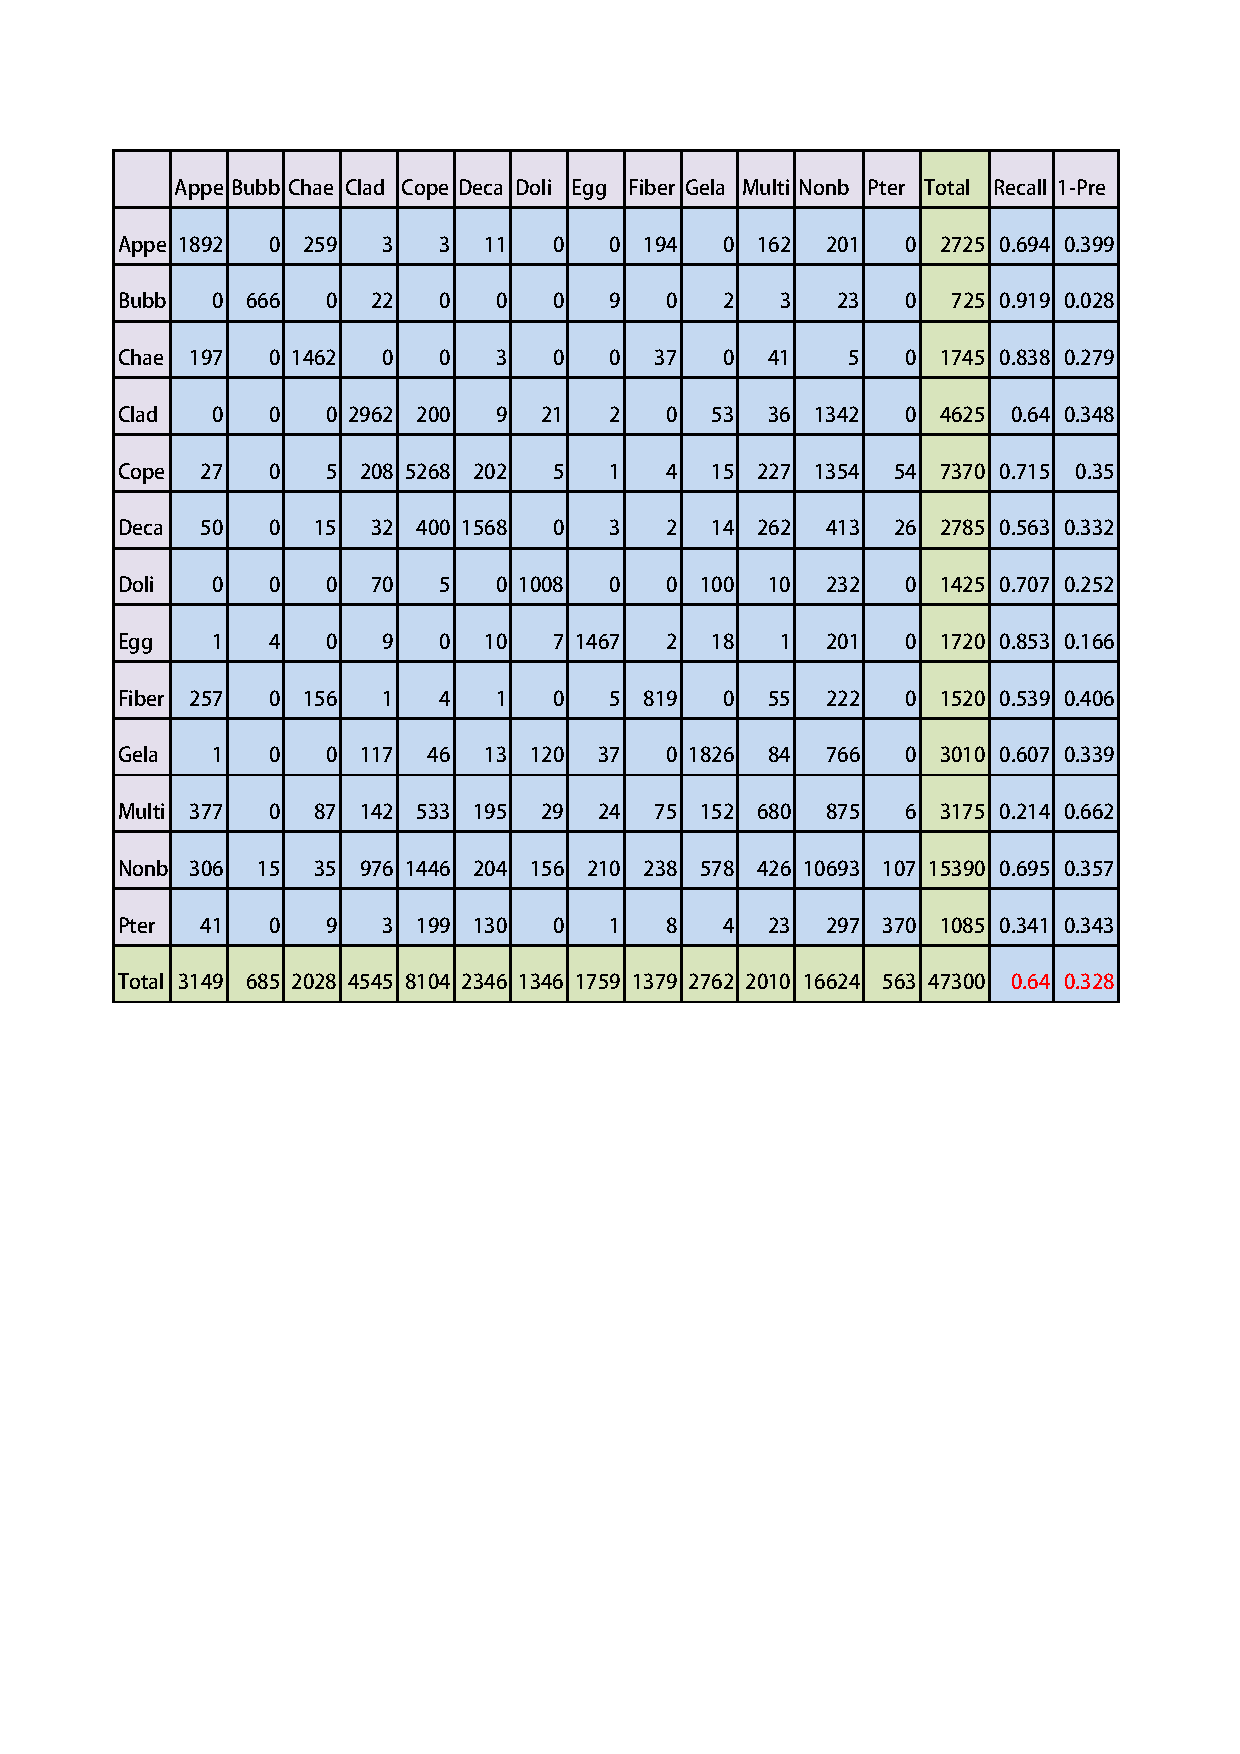
\includegraphics[width=1.0\linewidth]{LBP-SVM-2-folds-5-repetitions-32-256.pdf}
\end{tabular}
\label{LBP-SVM-2-folds-5-repetitions-32-256}
\end{table}

最后,对内距离形状上下文特征进行实验,我们用到的数据集中一共有13个不同种类的浮游动物,其中同一类中的图像在形状方面也有可能相差较大,这是由于数据集中的类别有的是在“门”、“属”、“目”等不同级别,有的级别下面还包含很多子级,不同的子级之间有可能差别很多,所以在提取内距离形状上下文特征选取模板时,通常不能每类只选一幅图像作为模板,这样会导致该类下的某些子级被忽略了,不能被正确分类。经过实验,我们得出结论:当从每类浮游动物图像中选取3幅及以上的图像作为一类的模板时,分类效果会比较好。对于提取的内距离形状上下文特征,我们分别利用支持向量机、随机森林、极限学习机分类器进行训练并在测试集上验证,最终发现极限学习机分类算法最适用于这一特征。当对每一类选取的模板数目增多时,分类效果会有所提升,但同时学习速度也会变慢,两者成反比的关系。

对此,我们进行了一些实验作说明。当每类浮游动物图像中挑选3张作为模板,一共选取39幅时,采用ELM进行训练,在测试集上的分类结果评价如表~\ref{IDSC-39-Features-MATLAB-ELM},其分类准确率为59.4\%。选取65幅图像作为模板时,评价结果如表~\ref{IDSC-65-Features-MATLAB-ELM},其分类准确率为65\%。模板数目增加到104张时,评价结果如表~\ref{IDSC-104-Features-MATLAB-ELM},其分类准确率为65.6\%。可以看到,当模板数目增多时,分类准确率是有所提高的,但同时出现的问题是运行速度会下降很多,要在既保证分类准确率又保证运行效率的情况下设定最佳模板数目。而对内距离形状上下文特征使用支持向量机和随机森林分类算法时效果都没有极限学习机好。

上述三类实验验证了每类特征所对应有效的分类算法,至此,分类器设计完成。

\begin{table}
\centering
\caption{提取内距离形状上下文特征并采用极限学习机进行分类的结果(39张图像作为模板)}
\begin{tabular}{c}
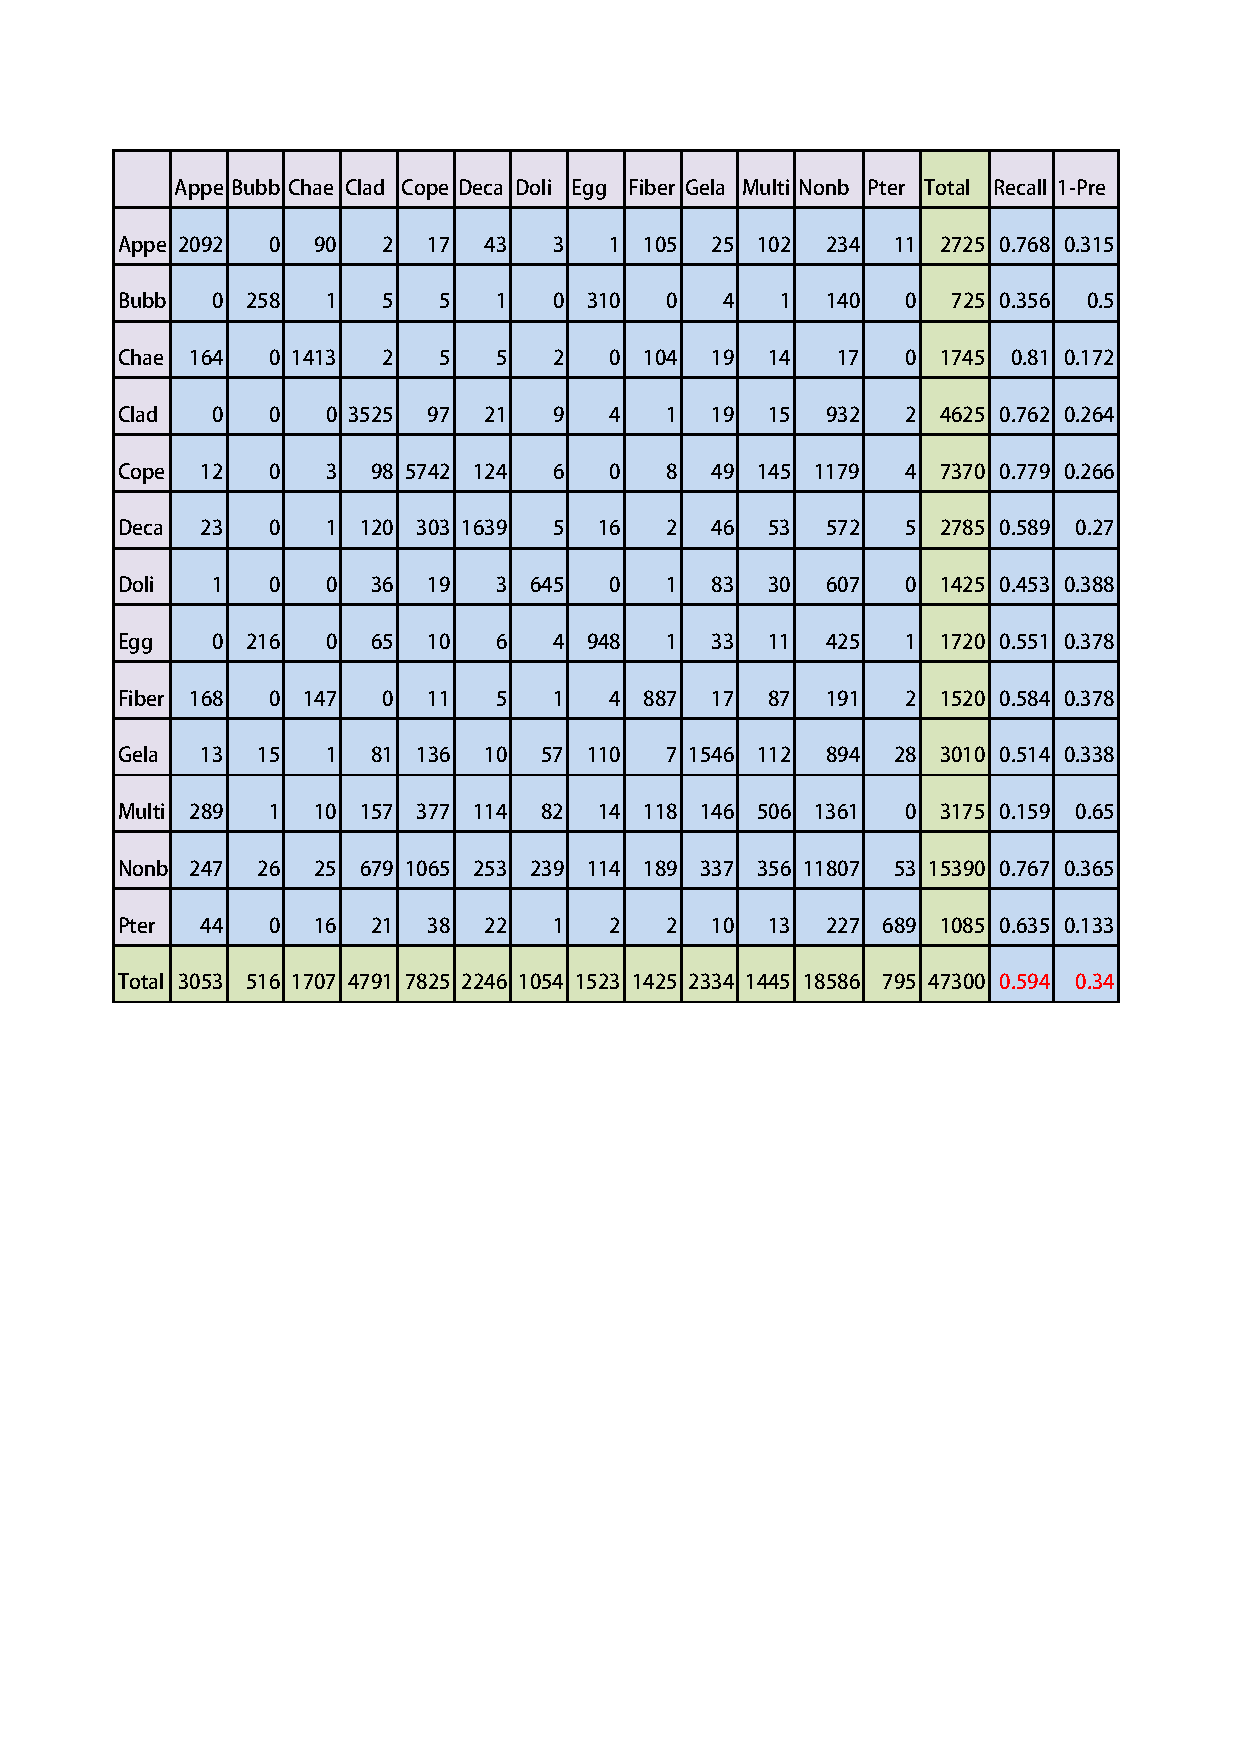
\includegraphics[width=1.0\linewidth]{IDSC-39-Features-MATLAB-ELM.pdf}
\end{tabular}
\label{IDSC-39-Features-MATLAB-ELM}
\end{table}

\begin{table}
\centering
\caption{提取内距离形状上下文特征并采用极限学习机进行分类的结果(65张图像作为模板)}
\begin{tabular}{c}
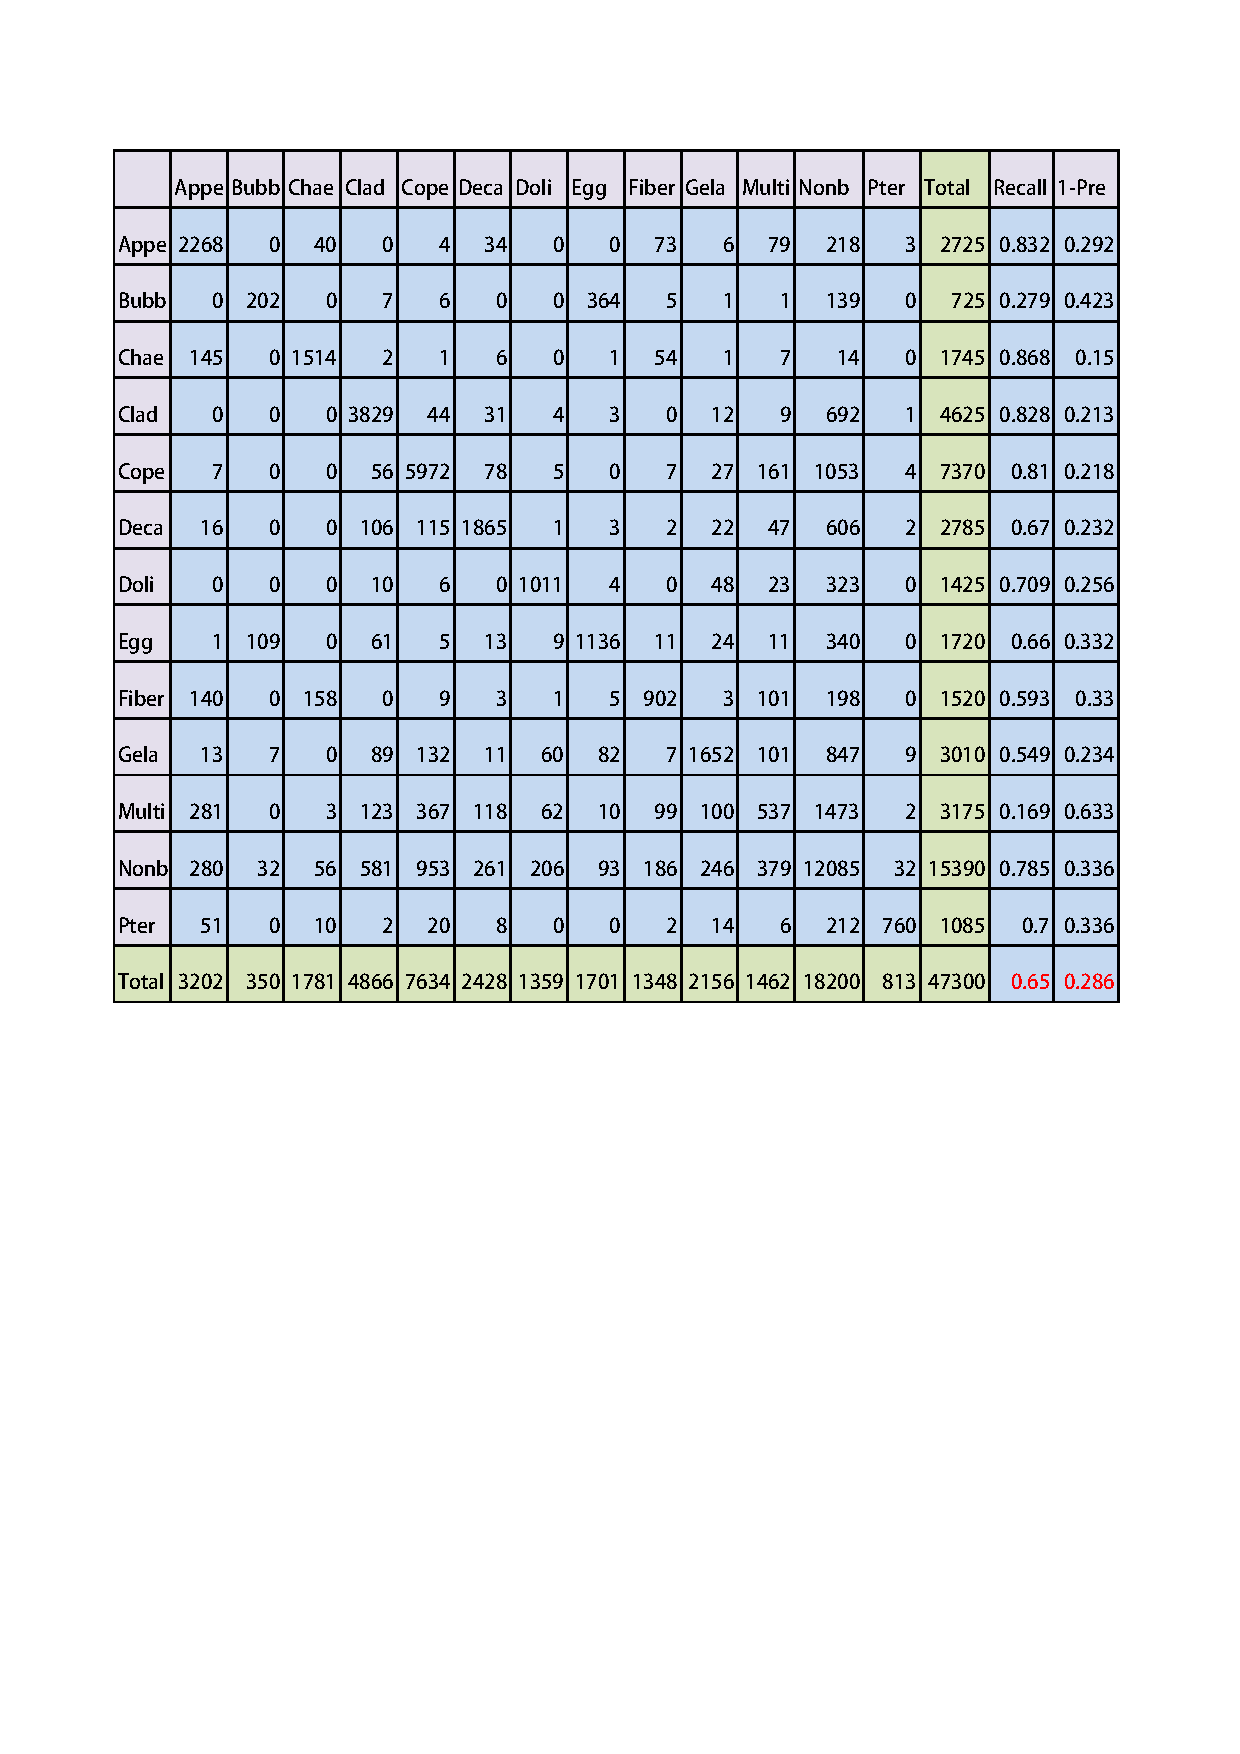
\includegraphics[width=1.0\linewidth]{IDSC-65-Features-MATLAB-ELM.pdf}
\end{tabular}
\label{IDSC-65-Features-MATLAB-ELM}
\end{table}

\begin{table}
\centering
\caption{提取内距离形状上下文特征并采用极限学习机进行分类的结果(104张图像作为模板)}
\begin{tabular}{c}
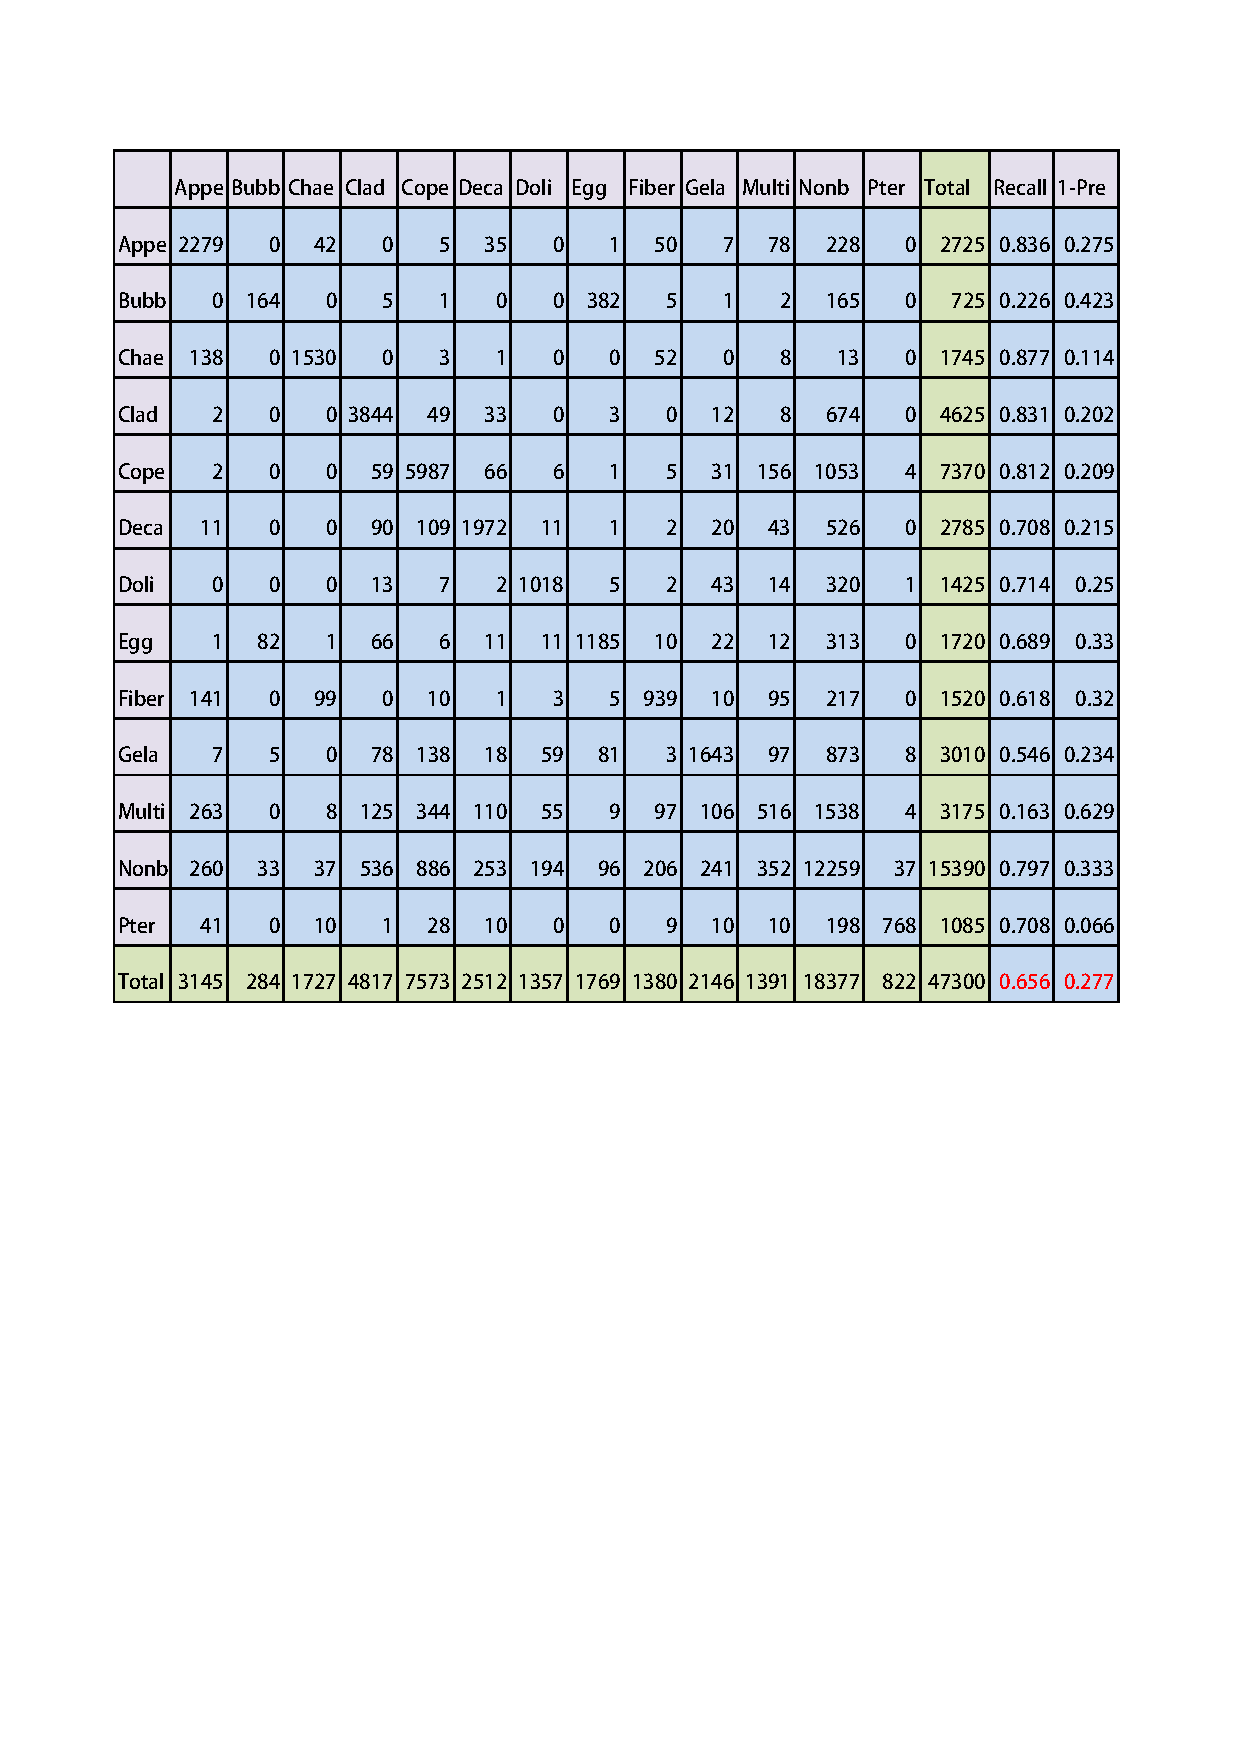
\includegraphics[width=1.0\linewidth]{IDSC-104-Features-MATLAB-ELM.pdf}
\end{tabular}
\label{IDSC-104-Features-MATLAB-ELM}
\end{table}


\chapter{多特征多分类器组合}

\section{基本原理}

本文选择了三类特征,对这三类特征分别用不同的分类算法进行分类,效果都不是很好,针对单个分类器不能完全表达浮游动物分类信息的情况,我们提出了一种基于多特征多分类器组合的浮游动物图像分类算法,框架如图~\ref{fig: framework}所示。首先,对浮游动物图像进行预处理以去除噪声。然后,对预处理后的图像提取三种不同类型的特征作为低层次特征。再将这些低层次特征输入到相应的机器学习算法,得到训练集中的每一幅图像在每一特征下被分到各个浮游生物图像类别中的概率,这个概率就作为中层次特征。最后,将三种类型特征对应的三种中层次特征串联起来并用支持向量机方法进行训练,得到最终的分类器。

\begin{figure}[!ht]
\centering
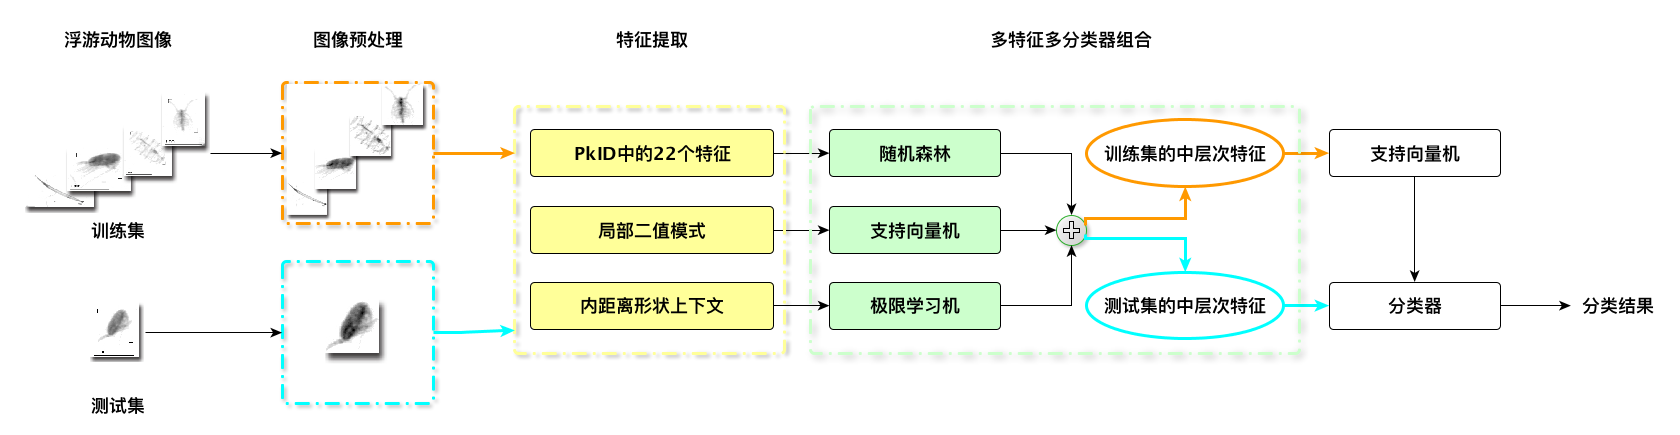
\includegraphics[width=1.0\linewidth]{framework.png}
\caption{基于多特征多分类器组合的浮游动物图像分类算法框架}
\label{fig: framework}
\end{figure}

在实验中,我们往往希望提取尽可能多的特征,以增强对图像或物体类别的描述,使分类效果更理想。但实际上特征数目与分类有效性之间并不是线性关系,很多特征本身可能只包含了少量有用信息,亦或者是带有一些冗余信息,这些都会对分类效果产生不好的影响。在第~\ref{3.1}和~\ref{2.3.3}节中,我们整理和总结了各种不同的特征,通过实验与分析,本文最终选取出的三类特征分别是PkID中的特征、局部二值模式和内距离形状上下文。

选取出特征后,我们采用多个分类器组合的技术对提取的不同类型的特征作不同的处理,每一类型的特征都用相应的适合该类型特征的分类算法来进行训练。如果训练集中有$M$幅图像,$n$个类别,我们提取了$m$种不同类型的特征,每一种类型的特征对应一种相应的分类算法,那么经过每一个分类算法除了能得到一个分类器外,还能得到训练集中的每一幅图像被分为每个类别的概率,对于整个数据集就会得到一个$M \times n$的矩阵,因为有$m$种不同类型的特征,所以最终会得到一个$M \times (n * m)$的矩阵。将这个矩阵作为对训练集图像提取的中层次特征,选取相应的分类算法进行训练,得到最终的分类器。

\section{图像预处理}

由于成像过程中受到的各种各样的干扰,我们所收集到的浮游图像不可避免地会带有一些噪声信号,这些噪声的引入,会直接导致图像的不清晰,造成识别准确率的下降。图~\ref{fig: origin_preprocess}(a)显示的是一幅原始的浮游动物图像,可以看到除了浮游动物目标外,周围还混杂了一些悬浮物、污点等噪声信息,对图像进行预处理的目的就是去除这些噪声信息,而保留和增强图像中对分类有用的信息。本文所采取的预处理方法是先对图像进行二值化,然后去除面积小于一定值的连通区域,图~\ref{fig: origin_preprocess}(b)显示的是经过预处理后的图像,除浮游动物外的一些污点噪声已经被去除掉了。

\begin{figure}[t]
  \centering%
  \begin{subfigure}{0.3\linewidth}
    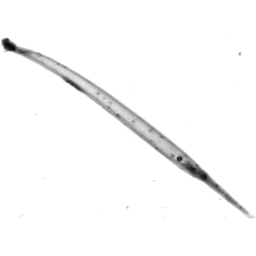
\includegraphics[height=4cm]{origin.png}
    \caption{}
  \end{subfigure}
  \hspace{4em}%
  \begin{subfigure}{0.3\linewidth}
    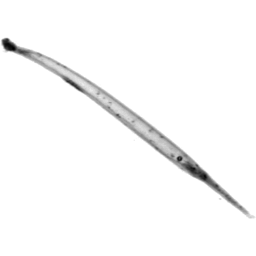
\includegraphics[height=4cm]{preprocess.png}
    \caption{}
  \end{subfigure}
  \caption{预处理前和预处理后的图像对比}
  \label{fig: origin_preprocess}
\end{figure}

\section{实验对比与分析}

在本文中,我们将所提出的基于多特征多分类器组合的浮游动物图像分类方法与ZooScan系统进行了对比,选用的数据集是~\ref{2.1}节中介绍的13类浮游动物图像集,评价方法采用的是$K$折交叉验证。

PkID软件中,有7种机器学习算法供选用,将所提取出的67个特征都用上,并且机器学习算法定为随机森林时,分类准确率最高,约为75\%,见表~\ref{PkID-RF}。

\begin{table}
\centering
\caption{PkID软件中随机森林分类器分类结果}
\begin{tabular}{c}
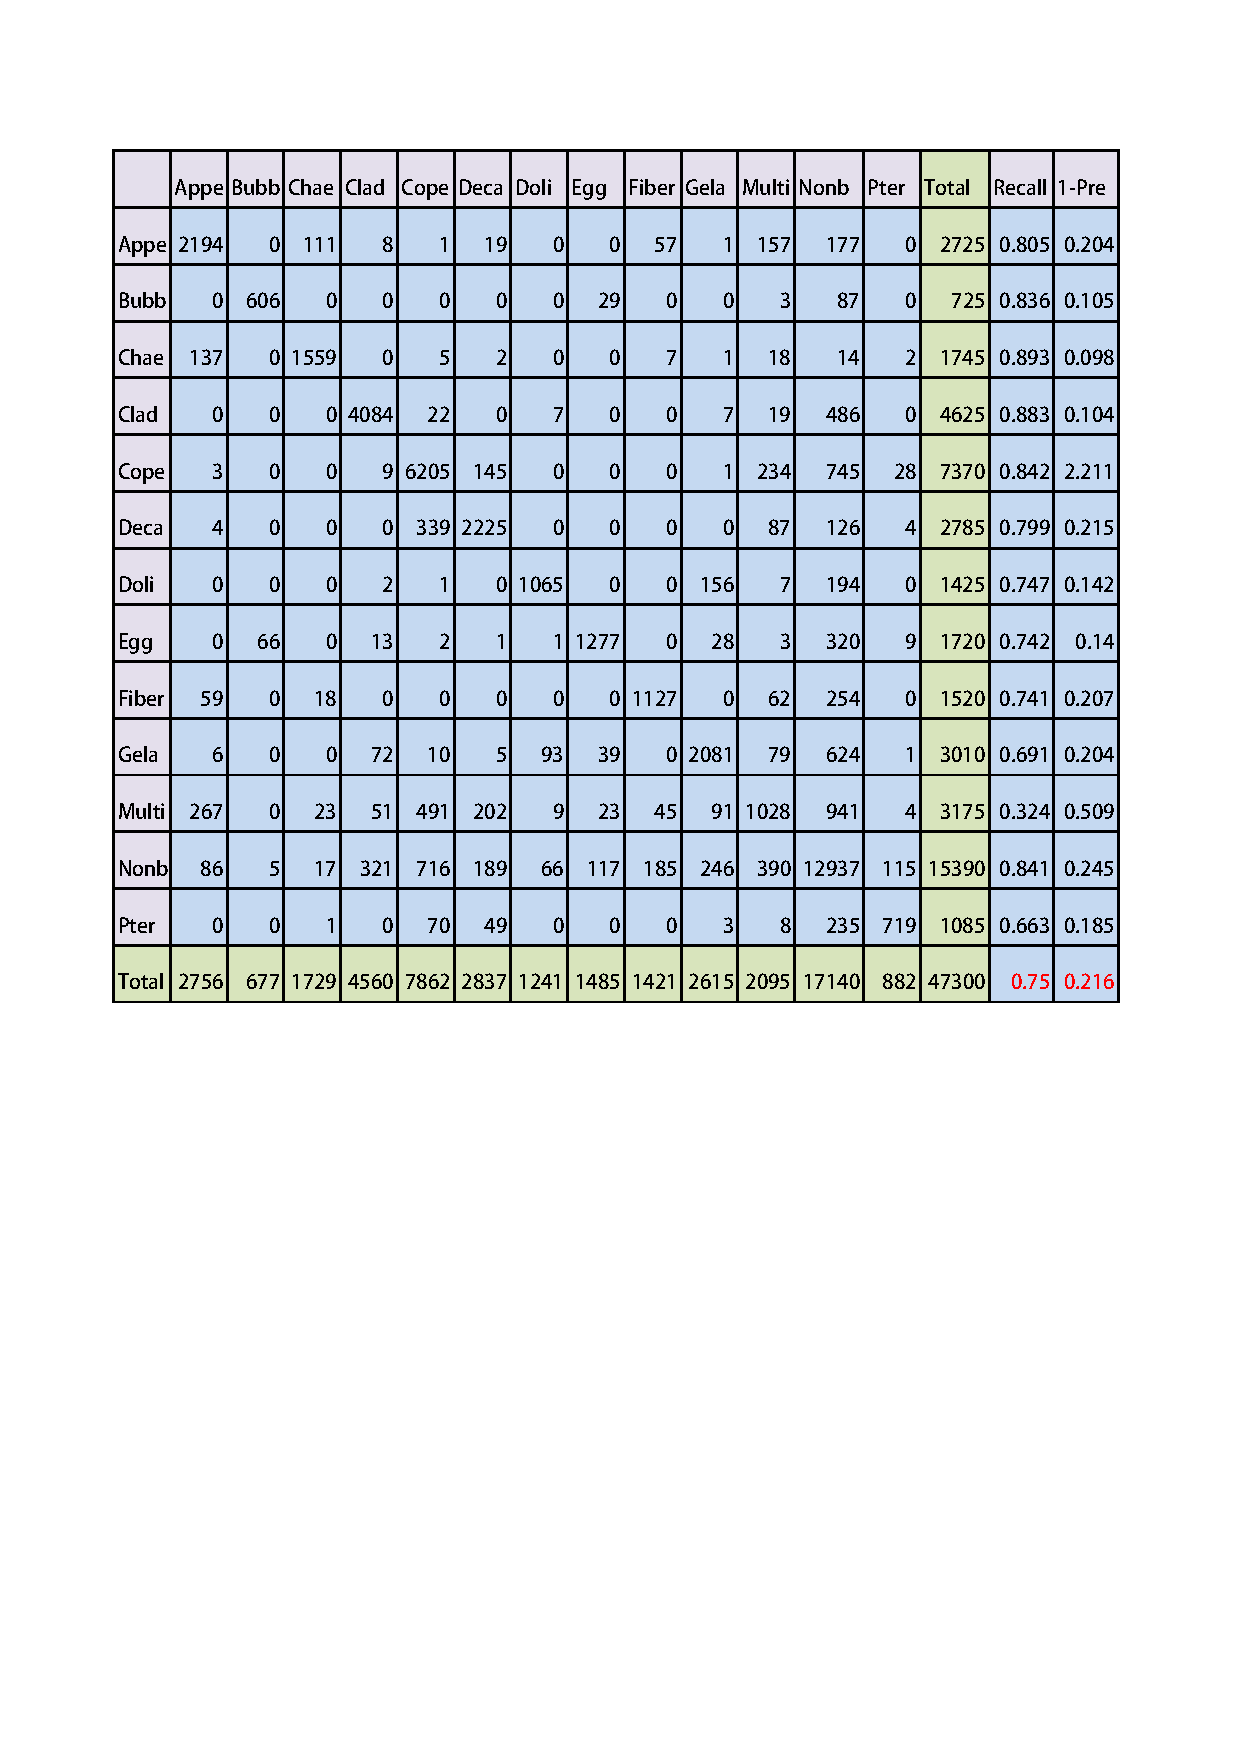
\includegraphics[width=1.0\linewidth]{PkID-RF.pdf}
\end{tabular}
\label{PkID-RF}
\end{table}

将我们的算法中得到的三个分类器特征(中层次特征)串联起来,输入到支持向量机分类算法中,得到最终的分类器。这里我们仍然对其中的内距离形状上下文的参数选取进行了一些实验。当内距离形状上下文特征中模板数目设为39时,得到的分类器对测试集的分类结果评价如表~\ref{20+IDSC39+LBP-Features-MATLAB}所示,其分类准确率为77.1\%。当内距离形状上下文特征中模板数目设为65时,得到的分类器对测试集的分类结果评价如表~\ref{20+IDSC65+LBP-Features-MATLAB}所示,其分类准确率为77.7\%。而当内距离形状上下文特征中模板数目设为104时,得到的分类器对测试集的分类结果评价如表~\ref{20+IDSC104+LBP-Features-MATLAB}所示,其分类准确率并没有变化,仍然为77.7\%。所以最终我们一般对内距离形状上下文特征中的模板数目设为65,这样既能在一定程度上提高分类准确率,又不会使运行速度变得过慢。

\begin{table}
\centering
\caption{多特征多分类器组合(内距离形状上下文特征采用39张图像作为模板)}
\begin{tabular}{c}
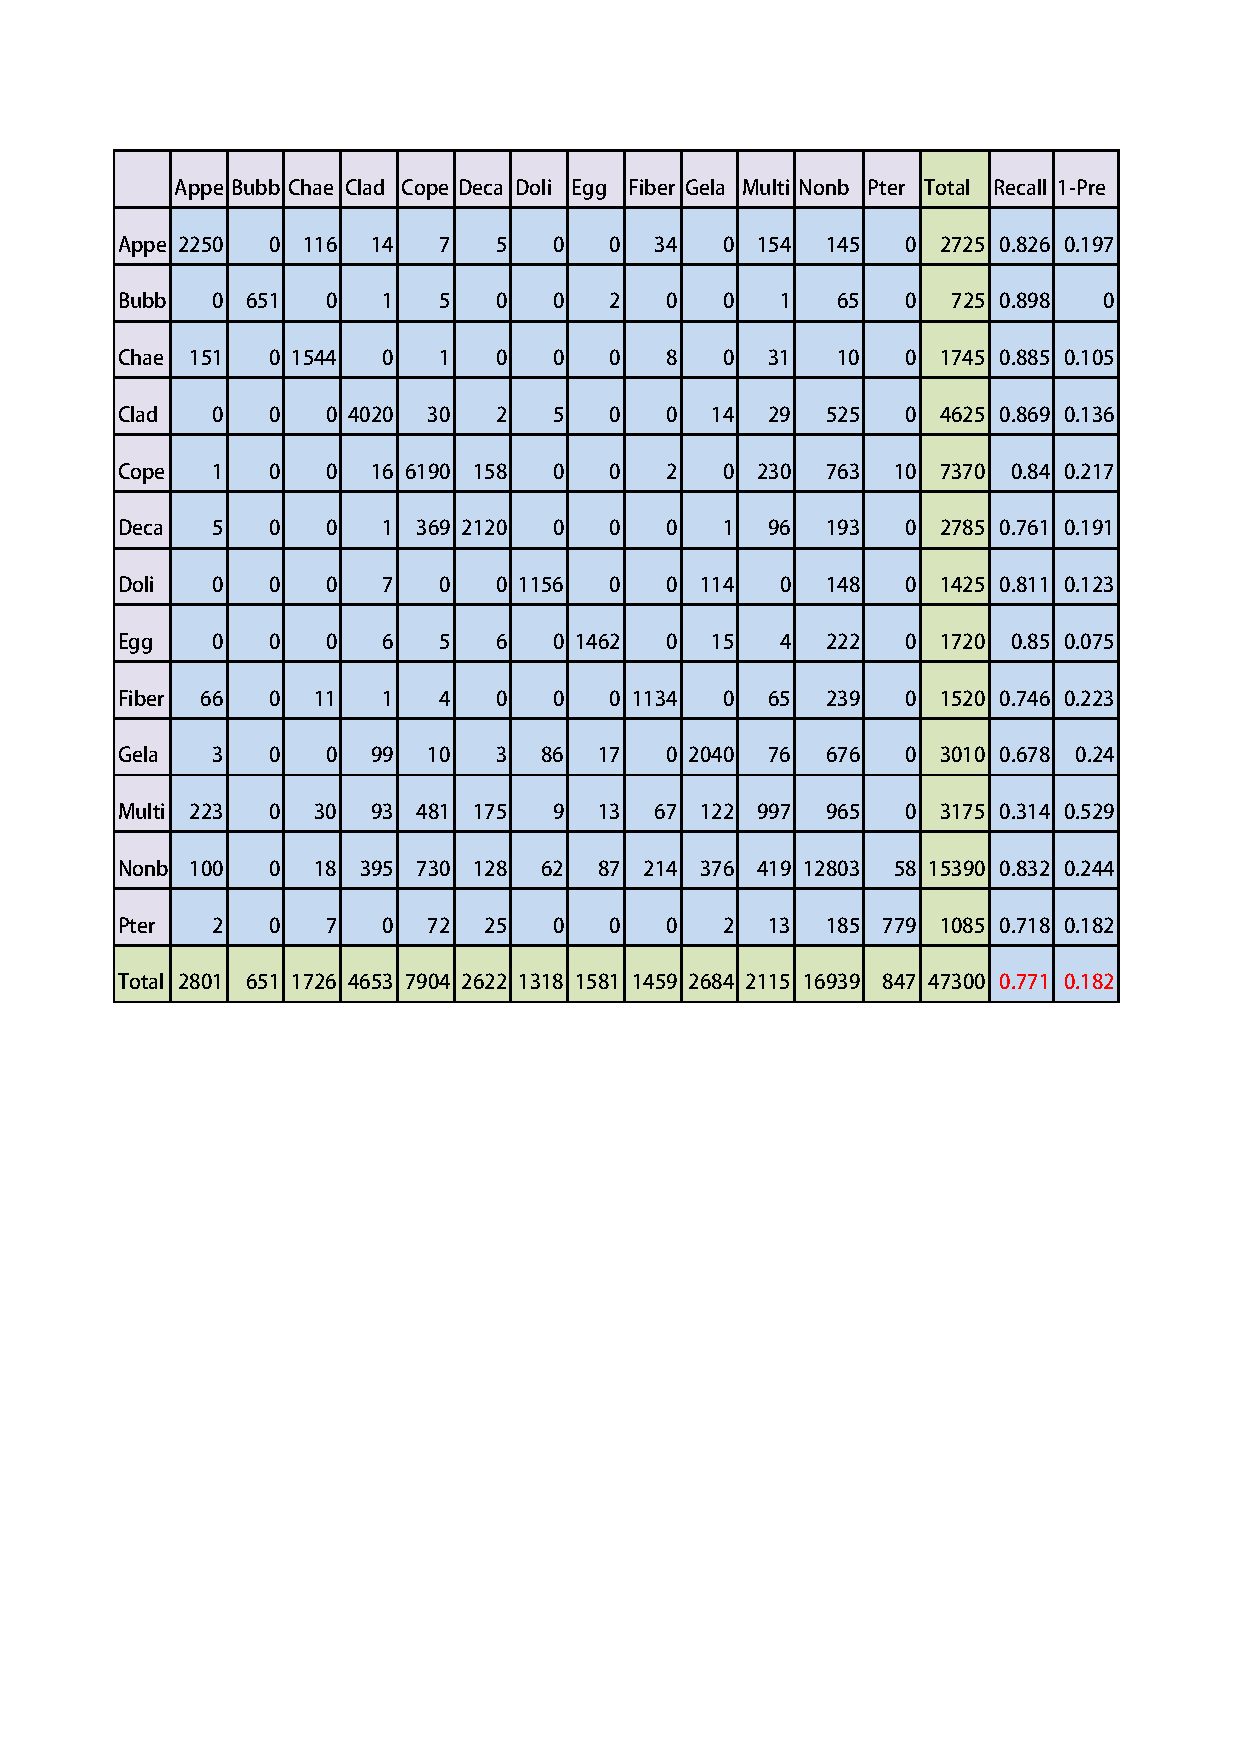
\includegraphics[width=1.0\linewidth]{20+IDSC39+LBP-Features-MATLAB.pdf}
\end{tabular}
\label{20+IDSC39+LBP-Features-MATLAB}
\end{table}

\begin{table}
\centering
\caption{多特征多分类器组合(内距离形状上下文特征采用65张图像作为模板)}
\begin{tabular}{c}
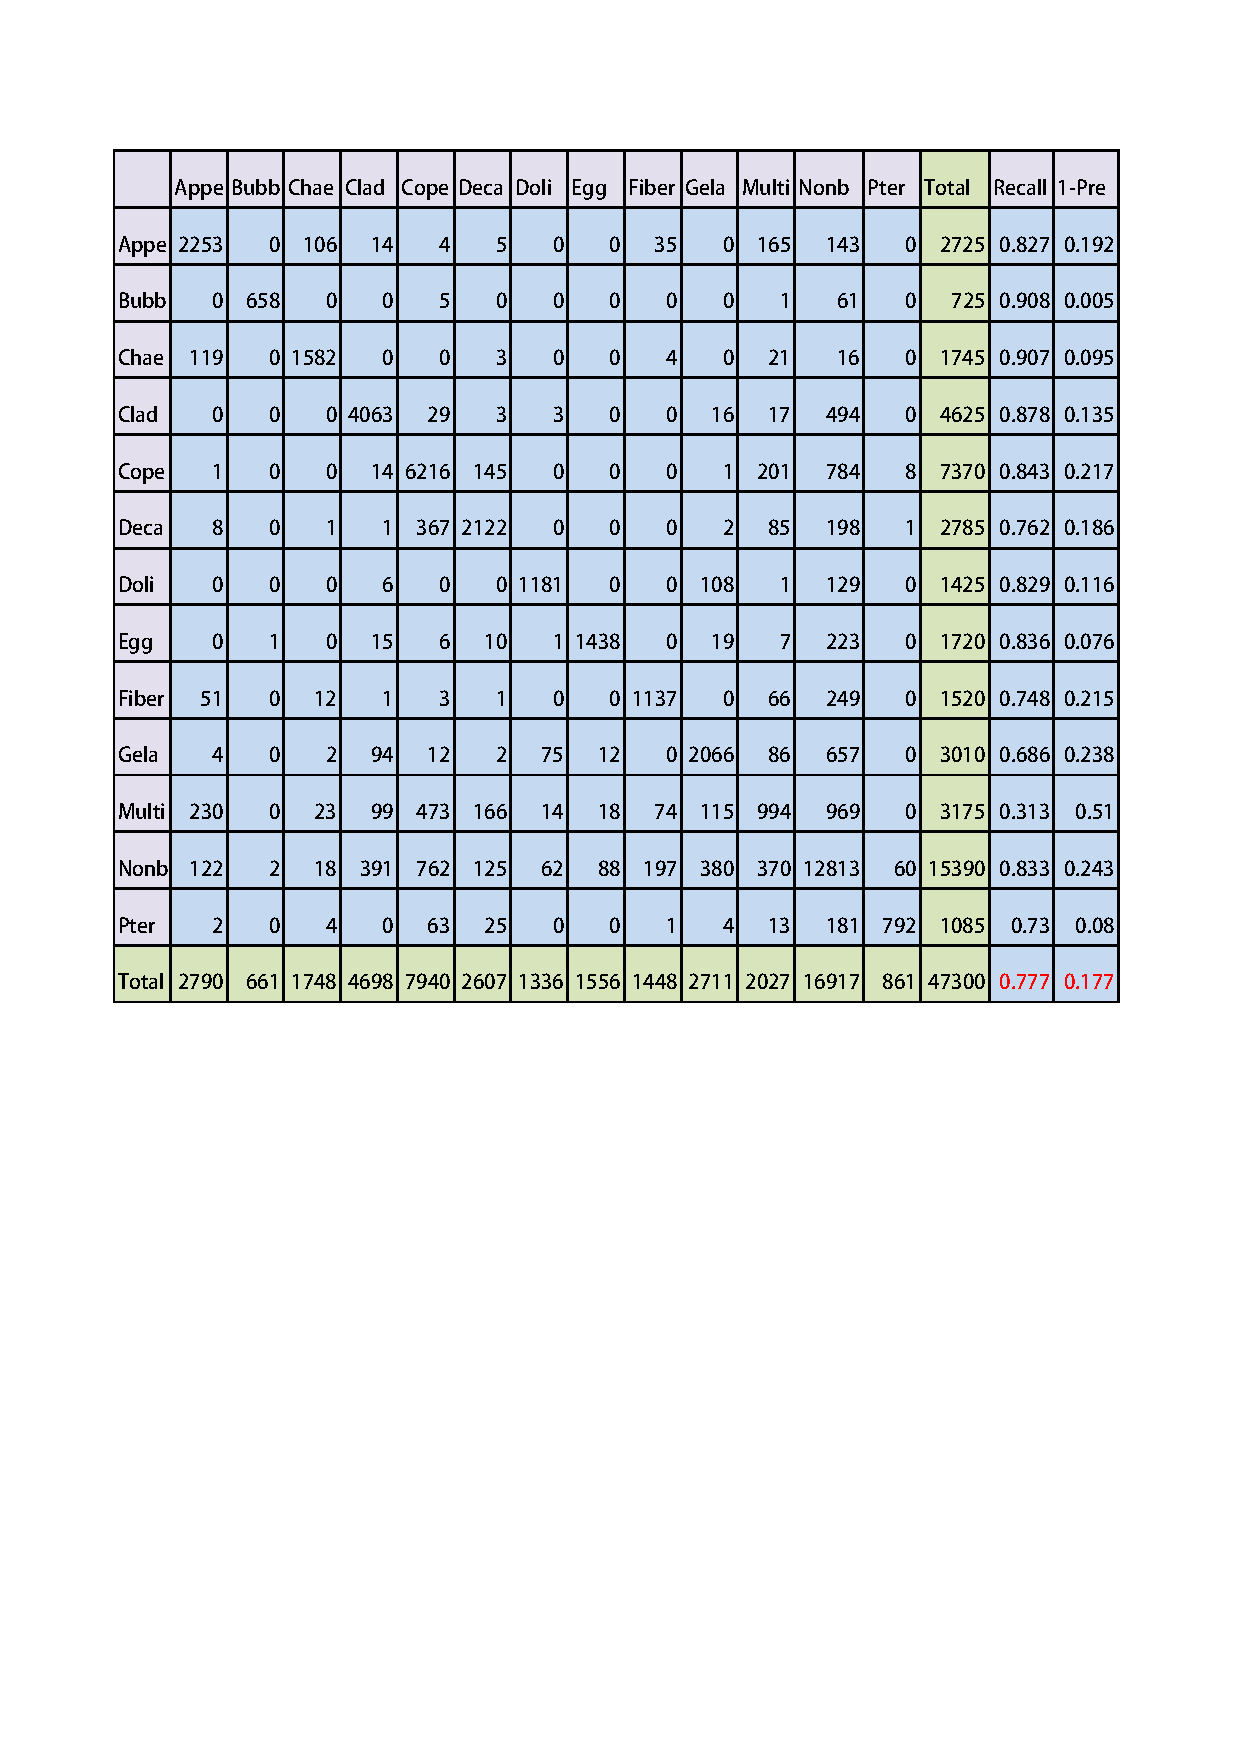
\includegraphics[width=1.0\linewidth]{20+IDSC65+LBP-Features-MATLAB.pdf}
\end{tabular}
\label{20+IDSC65+LBP-Features-MATLAB}
\end{table}

\begin{table}
\centering
\caption{多特征多分类器组合(内距离形状上下文特征采用104张图像作为模板)}
\begin{tabular}{c}
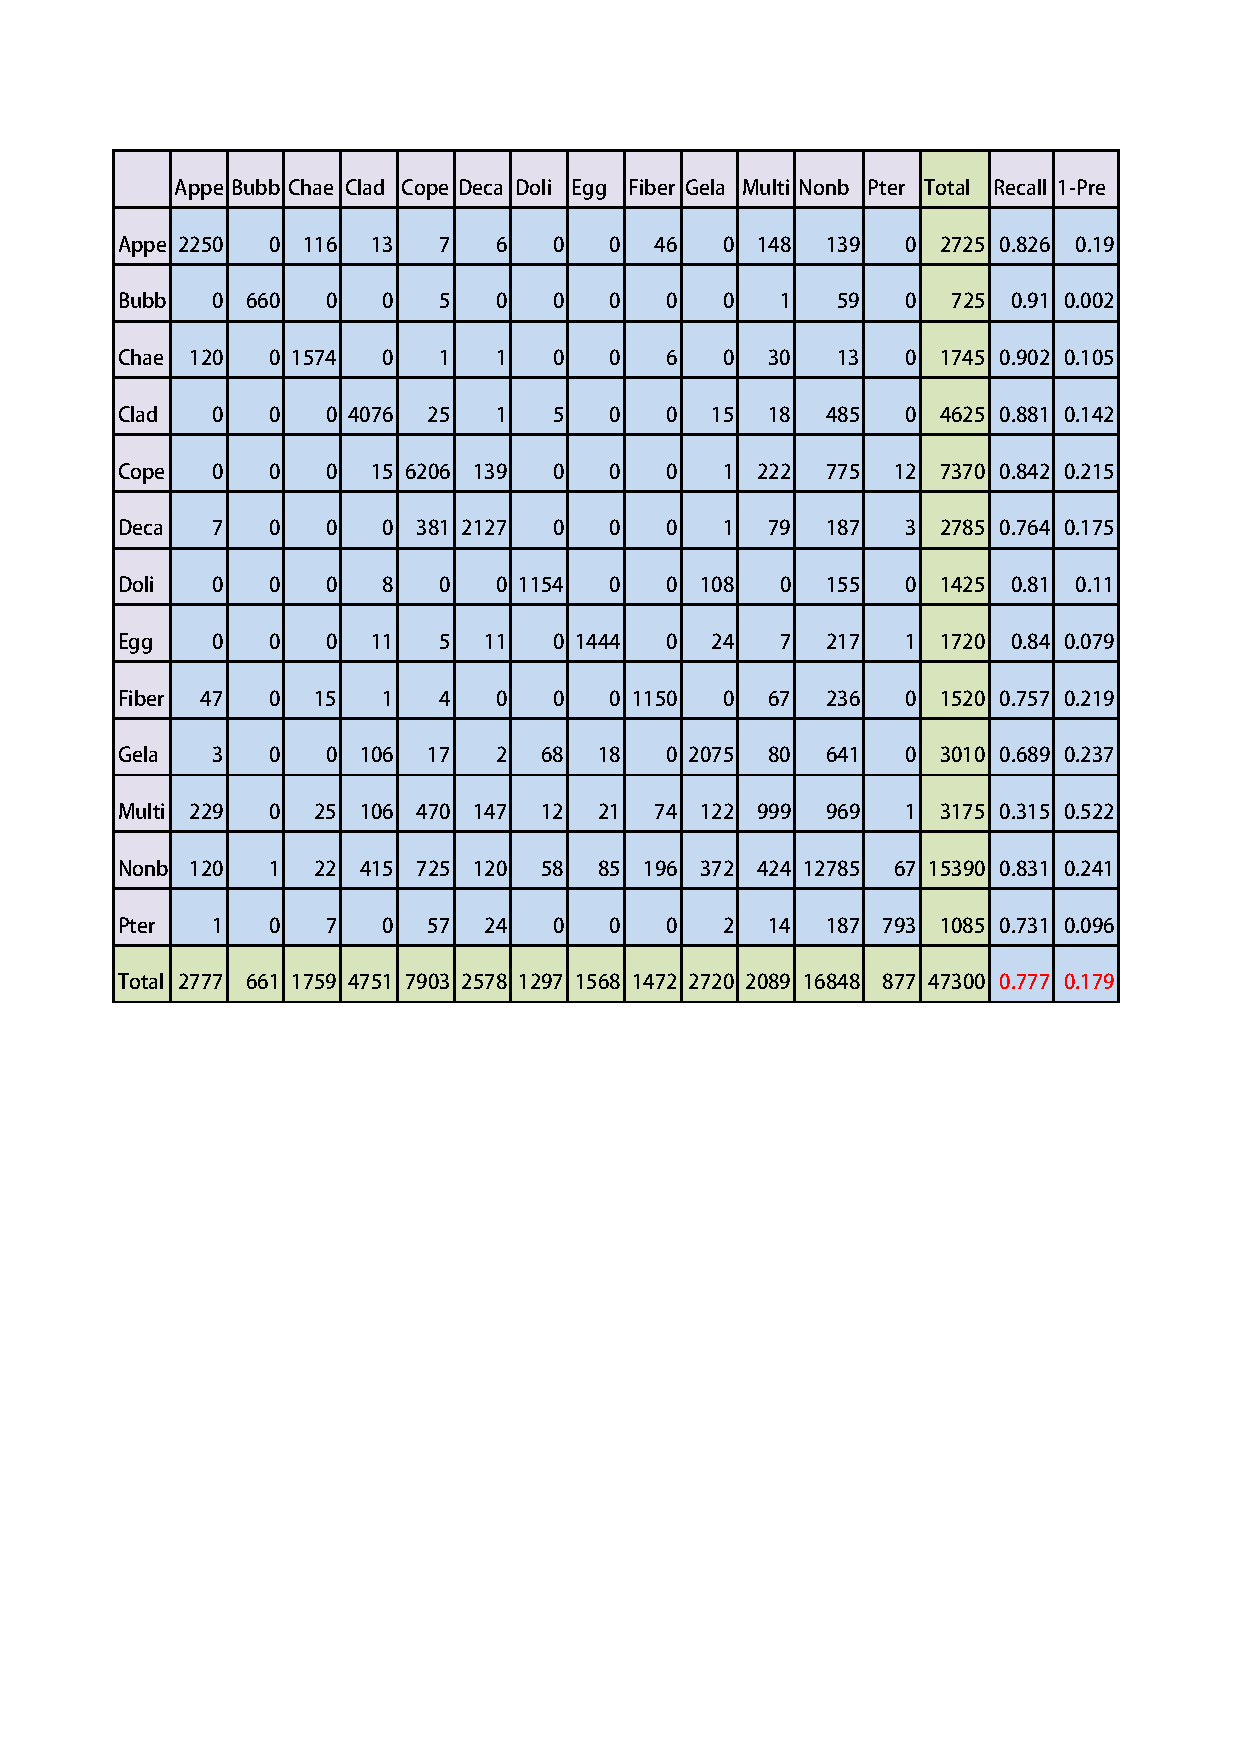
\includegraphics[width=1.0\linewidth]{20+IDSC104+LBP-Features-MATLAB.pdf}
\end{tabular}
\label{20+IDSC104+LBP-Features-MATLAB}
\end{table}

对比表~\ref{PkID-RF}和表~\ref{20+IDSC65+LBP-Features-MATLAB}可以看到,本文中所提出的基于多特征多分类器组合的浮游动物图像分类算法与ZooScan系统中的识别软件相比,在识别准确率上有了明显的提高。并且我们的方法在使用的特征数量上有所降低,只采用了24个特征。这24个特征又可以分为三类,对这三类特征分别利用不同的分类算法进行训练得到的单个分类器的分类效果比组合这三个分类器的效果要差,这是因为组合分类器正确利用了单个分类器提供的信息,从不同的角度反映了图像的特性,最终的结果表明本文提出的多特征多分类器组合的方法是有效的。

\chapter{总结与展望}

\section{总结}

浮游动物图像自动分类识别是浮游动物检测系统中的关键技术,随着浮游动物图像获取技术的不断提高,越来越多的图像数据被采集获取到,仅仅依赖人为的种类鉴别手段已经难以满足对大量数据进行实时快速处理的需要。基于机器学习方法的浮游动物图像分类方法,与其它方法相比,识别准确率更高,因此越来越受到重视。

本文围绕机器学习理论和多特征多分类器组合技术,进行了相关的研究和探索,主要完成了以下工作:

\begin{enumerate}
\item 以浮游生物成像系统和自动识别技术为基础,研究了国内外的发展现状,并且介绍了为什么要进行浮游动物图像分类识别的研究。
\item 对所要分类的浮游动物图像数据集进行了分析,对每类浮游动物的特点做了一个大致的整理,从而能够人为地对这些图像进行分类。
\item 对图像处理领域常用的特征以及在各种分类竞赛中所采用的一些经典特征做了总结,通过理论和实验的结合,从大量的特征中选择适用于浮游动物图像的特征。
\item 针对不同类型的特征,选择适用于该特征的分类算法进行分类器的设计。
\item 提出了一种基于多特征多分类器组合的浮游动物图像分类方法,从而能够综合不同分类器的信息,提高分类准确率。
\end{enumerate}

\section{展望}

尽管本文的算法在浮游动物的识别准确率上有所提高,并且对特征和分类器都进行了总结,做了大量的实验来验证哪些特征和分类器适用于解决浮游动物图像分类这类问题。但是还存在着一些不足,需要做进一步的研究:

\begin{enumerate}
\item 我们的算法是基于Matlab语言的,但Matlab在计算速度上仍然不够快,将来希望用C/C++语言进行编程,进一步提高算法的运行速度。
\item 本文采用的是对分类结果进行融合的方法,还有很多特征融合的方法没有进行尝试,下一步会针对特征融合进行研究,看看对识别效果有没有改善。
\item 每个类别图像数目相差较多时,识别准确率较低,当每个类别数目大致相同时,识别准确率会有所提高,后续会对这一现象继续研究,从理论和实验两方面来解释说明。
\item 由于我们的实验都是基于同一数据集的,可能会带有数据集偏见,今后的研究希望能不依赖于数据集,要找到在各种浮游动物图像数据集上都能取得较好效果的特征和分类器。
\end{enumerate}

%%% 其它部分
\backmatter

% 本科生要这几个索引,研究生不要。选择性留下。
\makeatletter
\ifthu@bachelor
  % 插图索引
  \listoffigures
  % 表格索引
  \listoftables
  % 公式索引
  %\listofequations
\fi
\makeatother


% 参考文献
\bibliographystyle{thubib}
\bibliography{ref/refs}


% 致谢
%%% Local Variables:
%%% mode: latex
%%% TeX-master: "../main"
%%% End:

\begin{ack}
时光匆匆如流水,转眼便又是毕业时节了,在我三年的硕士研究生生涯里,我所收获的不仅仅是愈加丰厚的知识,更重要的是思维方式和表达能力的转变与提升。我很庆幸在这三年我遇到了很多的良师益友,无论在学习上、生活上还是工作上,都给予了我无私的帮助和悉心的照顾,让我在一个温馨、有爱的环境中度过了我的三年研究生生活。

首先,我要感谢我的导师郑海永,这三年来给我最多教育和帮助的人!从我开始读研开始,郑老师一直对我严格要求,在他的指导下,我不仅树立了远大的学习目标,掌握了基本的研究方法,还明白了很多为人处世的道理。本论文从选题到最终完成,每一步都得到了郑老师的帮助和指点,在我迷茫时给予适时的鼓励,帮助我开拓研究思路,解决问题。感谢师母冯丽颖的关怀和教育,使我认识到自身的不足,从而努力提高自己,做一个坚强、会生活、懂生活的新时代女性。在此,谨向导师和师母表示崇高的敬意和衷心的感谢!

感谢实验室所有兄弟姐妹,没有你们的陪伴,我不会拥有这么美好、难忘的三年回忆。感谢我的师姐赵红苗、师妹王如晨,和我并肩作战,在我的研究课题上给予了很多的支持和帮助,让我有了更大提高。

感谢我的家人,谢谢你们无私的付出,在我身后坚定地支持我、关心我、帮助我,有你们在,我更安心!

感谢国家自然科学基金青年科学基金项目“基于视觉注意结合生物形态特征的海洋浮游植物显微图像分析”(批准号:61301240)、国家自然科学基金项目“基于生物形态特征的中国海常见有害赤潮藻显微图像识别”(批准号:61271406)和中央高校基本科研业务费“海洋浮游动物原位探测与分析系统”(批准号:201562023)的资助。

最后,感谢所有关心和帮助过我的人,祝愿你们幸福安康!
\end{ack}


% 附录
%\begin{appendix}
%%%% Local Variables: 
%%% mode: latex
%%% TeX-master: "../main"
%%% End: 

\chapter{}
\label{}

\chapter{}
\section{}

\chapter{}


%\end{appendix}

% 个人简历
\begin{resume}

  \resumeitem{个人简历}

  1990 年 9 月 4 日出生于 江苏 省 泰州 市 姜堰 区。
  
  2009 年 9 月考入 中国海洋大学 电子工程系 电子信息科学与技术 专业,2013 年 6 月本科毕业并获得 理学 学士学位。
  
  2013 年 9 月考入 中国海洋大学 电子 系攻读 硕士 学位至今。

  \resumeitem{发表的学术论文} % 发表的和录用的合在一起
     
  \begin{enumerate}[{[}1{]}]
  \item Wang X, Dai J, Zhu Y, Zheng H and Qiao X. Spectral saliency via automatic adaptive amplitude spectrum analysis. Journal of Electronic Imaging, 2016. (SCI 收录)
  \item Zhu Y, Chang L, Dai J, Zheng H, Zheng B. Automatic object detection and segmentation from underwater images via saliency-based region merging. Proceedings of OCEANS 2016 MTS/IEEE Shanghai, 2016. (EI 收录)
  \end{enumerate}

  \resumeitem{在学期间参加的研究项目} % 有就写,没有就删除
  \begin{enumerate}
  \item 国家自然科学基金青年科学基金项目“基于视觉注意结合生物形态特征的海洋浮游植物显微图像分析”(批准号:61301240)
  \item 国家自然科学基金项目“基于生物形态特征的中国海常见有害赤潮藻显微图像识别”(批准号:61271406)
  \item 中央高校基本科研业务费“海洋浮游动物原位探测与分析系统”(批准号:201562023)
  \end{enumerate}
  
\end{resume}

\end{document}
